\documentclass[12pt, titlepage]{article}

\usepackage{booktabs}
\usepackage{tabularx}
\usepackage{hyperref}
\hypersetup{
    colorlinks,
    citecolor=black,
    filecolor=black,
    linkcolor=red,
    urlcolor=blue
}
\usepackage[round]{natbib}
\usepackage{adjustbox}
\usepackage[dvipsnames]{xcolor}
\usepackage{float}
\usepackage{changepage}
\usepackage{pdflscape}


%% Comments

\usepackage{color}

\newif\ifcomments\commentstrue %displays comments
%\newif\ifcomments\commentsfalse %so that comments do not display

\ifcomments
\newcommand{\authornote}[3]{\textcolor{#1}{[#3 ---#2]}}
\newcommand{\todo}[1]{\textcolor{red}{[TODO: #1]}}
\else
\newcommand{\authornote}[3]{}
\newcommand{\todo}[1]{}
\fi

\newcommand{\wss}[1]{\authornote{blue}{SS}{#1}} 
\newcommand{\plt}[1]{\authornote{magenta}{TPLT}{#1}} %For explanation of the template
\newcommand{\an}[1]{\authornote{cyan}{Author}{#1}}

%% Common Parts

\newcommand{\progname}{Software Eng} % PUT YOUR PROGRAM NAME HERE
\newcommand{\authname}{Team \#, Team Name
\\ Student 1 Matthew Collard
\\ Student 2 Sam Gorman
\\ Student 3 Ethan Kannampuzha
\\ Student 4 Kieran Gara} % AUTHOR NAMES                  

\usepackage{hyperref}
    \hypersetup{colorlinks=true, linkcolor=blue, citecolor=blue, filecolor=blue,
                urlcolor=blue, unicode=false}
    \urlstyle{same}
                                


\begin{document}

\title{Verification and Validation Report: \progname} 
\author{\authname}
\date{\today}
	
\maketitle

\pagenumbering{roman}

\section{Revision History}

\begin{tabularx}{\textwidth}{p{3cm}p{2cm}X}
\toprule {\bf Date} & {\bf Version} & {\bf Notes}\\
\midrule
March 6, 2024 & 1.0 & Team worked all together on filling in all sections for revision 0 report\\
\bottomrule
\end{tabularx}

~\newpage

\section{Symbols, Abbreviations and Acronyms}

\renewcommand{\arraystretch}{1.2}
All  symbols, abbreviations, and acronyms can be found in section 1.4 of the  \href{https://github.com/SammyG7/Mac-AR/blob/main/docs/SRS/SRS.pdf}{SRS}.


\newpage

\tableofcontents

\listoftables %if appropriate

\newpage

\pagenumbering{arabic}

This document outlines the results of implementing the verification and validation plan. Included is a summary of all manual and automated tests performed on the project, along with their outputs. Any tests marked with "TBD"

\section{Functional Requirements Evaluation}

\subsection{Game Room Testing}
The following section goes over tests related to starting a game, loading game assets, and determining/displaying puzzles.


Table \ref{table:GR1} and \ref{table:GR2} below demonstrates the functional requirements evaluation for the game room. The way the game room will be assessed will be through the use of manual testing.

\begin{table}[H]
\caption{\bf Functional Requirements Evaluation Results for Game Room Testing}
\resizebox{6in}{!}{\begin{tabular}{|l|p{0.15\linewidth}|p{0.3\linewidth}|p{0.3\linewidth}|p{0.3\linewidth}|p{0.1\linewidth}|}
\hline
\multicolumn{1}{|l|}{\bfseries Id} & \multicolumn{1}{|l|}{\bfseries Type} & \multicolumn{1}{l|}{\bfseries Inputs} & \multicolumn{1}{l|}{\bfseries Expected Result} & \multicolumn{1}{l|}{\bfseries Actual Result} & \multicolumn{1}{l|}{\bfseries Result}\\
\hline
Test-CR1 & Manual & User presses Host button. & User redirected to create game menu which has entries to set game room settings (game room name, game room capacity, game room password). & Same as expected & \textcolor{Green}{Pass} \\
\hline
Test-CR2 & Manual & Game room name inputted. The game room name will be
a string consisting of letters, numbers, and ascii characters, and of
character length greater than 3 and less than 64. & Game room with specified name is created in database. & Same as expected & \textcolor{Green}{Pass} \\
\hline
Test-CR3 & Manual & User tries to create a new game room without inputting a name for the game room & Game room is not created and error message tells user that game room name is not valid. & Same as expected & \textcolor{Green}{Pass} \\
\hline
Test-CR4 & Manual &  User slides game room capacity slider to adjust game room capacity (min 2, max 10)  & Game room with specified capacity is created in database. & Same as expected & \textcolor{Green}{Pass} \\
\hline
Test-CR5 & Manual & User inputs game room password. The password length will be between 8 and 64 characters, and consists of letters, number, and ASCII characters arranged in a random order.  & Game room requiring password specified by user is created in database. & Same as expected & \textcolor{Green}{Pass} \\
\hline
Test-CR6 & Manual & User does not input anything for game room password, and hosts a game room.  & Game room requiring no password is created in database. & Same as expected & \textcolor{Green}{Pass} \\
\hline
\end{tabular}}
\label{table:GR1}
\end{table}

\begin{table}[H]
\caption{\bf Functional Requirements Evaluation Results for Game Room Testing 2}
\resizebox{6in}{!}{\begin{tabular}{|l|p{0.15\linewidth}|p{0.3\linewidth}|p{0.3\linewidth}|p{0.3\linewidth}|p{0.1\linewidth}|}
\hline
\multicolumn{1}{|l|}{\bfseries Id} & \multicolumn{1}{|l|}{\bfseries Type} & \multicolumn{1}{l|}{\bfseries Inputs} & \multicolumn{1}{l|}{\bfseries Expected Result} & \multicolumn{1}{l|}{\bfseries Actual Result} & \multicolumn{1}{l|}{\bfseries Result}\\
\hline
Test-JR1 & Manual & User presses Join Game button  & User redirected to join room menu which lists all present game rooms in database that are available to be joined and are under capacity. & Same as expected & \textcolor{Green}{Pass} \\
\hline
Test-JR2 & Manual & User attempts to enter a game room at maximum capacity. & User is not able to join the game room. & Same as expected & \textcolor{Green}{Pass} \\
\hline
Test-JR3 & Manual & User enters room name of a created room that has no password set. & User joins game room and available capacity decreases by 1. & Same as expected & \textcolor{Green}{Pass} \\
\hline
Test-JR4 & Manual & User enters room name and password of created game room. & User joins game and available capacity decreases by 1. & Same as expected & \textcolor{Green}{Pass} \\
\hline
Test-JR5 & Manual & User enters room name and password of created game room & User is redirected to game room menu which displays the users present in the game room. & Same as expected & \textcolor{Green}{Pass} \\
\hline
Test-RS1 & Manual & User presses settings button, then processes to change the game
room name, password, or capacity. & User is redirected to edit game settings menu which displays the current settings of the game room (ie. room capacity, and password). & Same as expected & \textcolor{Green}{Pass} \\
\hline
Test-RS2 & Manual & Password to game room is updated. & Game room is updated to require the new password. & Same as expected & \textcolor{Green}{Pass} \\
\hline
Test-RS3 & Manual & Game room settings are changed. & Game room settings menu is updated to show current setting values. & Same as expected & \textcolor{Green}{Pass} \\
\hline
Test-ER1 & Manual & Game room menu is present and user presses exit button. & User is removed from game room. & Same as expected & \textcolor{Green}{Pass} \\
\hline
Test-ER2 & Manual & User exits game room. & Game room menu updated to no longer display the user in
the game room. & Same as expected & \textcolor{Green}{Pass} \\
\hline
Test-ER3 & Manual & User exits game room. & Total number of users in game room decreases by one. & Same as expected & \textcolor{Green}{Pass} \\
\hline
\end{tabular}}
\label{table:GR2}
\end{table}

\subsection{Start Game Testing}
The following section goes over tests related to starting a game, loading game assets, and determining/displaying puzzles.

\begin{table}[H]
\caption{\bf Functional Requirements Evaluation Results for Start Game Testing}
\resizebox{6in}{!}{\begin{tabular}{|l|p{0.15\linewidth}|p{0.3\linewidth}|p{0.3\linewidth}|p{0.3\linewidth}|p{0.1\linewidth}|}
\hline
\multicolumn{1}{|l|}{\bfseries Id} & \multicolumn{1}{|l|}{\bfseries Type} & \multicolumn{1}{l|}{\bfseries Inputs} & \multicolumn{1}{l|}{\bfseries Expected Result} & \multicolumn{1}{l|}{\bfseries Actual Result} & \multicolumn{1}{l|}{\bfseries Result}\\
\hline
Test-ST1 & Manual & User presses start button & Game is started & Same as expected & \textcolor{Green}{Pass} \\
\hline
Test-ST2 & Manual & User starts game & First puzzle GameObject is instantiated and loaded into the scene & Same as expected & \textcolor{Green}{Pass} \\
\hline
Test-ST3 & Automated & User starts game & Order of puzzles is determined and each user is assigned a part of the puzzle & Same as expected & \textcolor{Green}{Pass} \\
\hline
Test-ST4 & Automated &  User starts game & Progress bar displayed on screen to let user know current progress & TBD & \textcolor{Red}{TBD} \\
\hline
Test-ST5 & Automated & User starts game  & Puzzle is displayed to each user and game commences & Same as expected & \textcolor{Green}{Pass} \\
\hline
\hline
\end{tabular}}
\label{table:ST1}
\end{table}

\subsection{Puzzle Interaction Testing}
The following section goes over tests related to interacting with the puzzle UI elements and the corresponding updated on the back end.

\begin{table}[H]
\caption{\bf Functional Requirements Evaluation Results for Puzzle Interaction Testing}
\resizebox{6in}{!}{\begin{tabular}{|l|p{0.15\linewidth}|p{0.3\linewidth}|p{0.3\linewidth}|p{0.3\linewidth}|p{0.1\linewidth}|}
\hline
\multicolumn{1}{|l|}{\bfseries Id} & \multicolumn{1}{|l|}{\bfseries Type} & \multicolumn{1}{l|}{\bfseries Inputs} & \multicolumn{1}{l|}{\bfseries Expected Result} & \multicolumn{1}{l|}{\bfseries Actual Result} & \multicolumn{1}{l|}{\bfseries Result}\\
\hline
Test-PI1 & Manual & User Selects Puzzle & Puzzle Enlarges On UI & TBD & \textcolor{Red}{TBD} \\
\hline
Test-PI2 & Manual & User taps a key on the Combination Puzzle & If the digit was correct, the digit appears on the screen, if it was not, the combination puzzle turns red & Same as expected & \textcolor{Green}{Pass} \\
\hline
Test-PI2 & Manual & User presses a coloured button on the Simon Says Puzzle & If the colour pressed was the correct one, the system awaits the next button press. If it was not, the level is set to one, and the colour combination gets re-transmitted on the cube. & Same as expected & \textcolor{Green}{Pass} \\
\hline
Test-PI2 & Manual & User rotates their phone on the maze puzzle & The maze rotates in accordance with the phone rotation & Same as expected & \textcolor{Green}{Pass} \\
\hline
Test-PI2 & Manual & User performs drags a wire on the Wires Puzzle & The wire follows the drag, and locks onto a node if the user lets go of their finger over it & Same as expected & \textcolor{Green}{Pass} \\
\hline
Test-PI2 & Manual & User types on the input field of the Isometric Puzzle & The input field updates on all the user's screen. If the code was entered correctly, the puzzle is completed. & Same as expected & \textcolor{Green}{Pass} \\
\hline
Test-PI3 & Automated & User performs an action on a puzzle & Puzzle back end information is updated appropriately to action & Same as expected & \textcolor{Green}{Pass} \\
\hline
Test-PI4 & Manual & User performs an action on a puzzle & Puzzle UI updates appropriately for other members in game room  & Same as expected & \textcolor{Green}{Pass} \\
\hline
Test-PI5 & Manual & Multiple users perform actions to complete puzzle & All users notified puzzle that has been completed and game room progresses &  Same as expected& \textcolor{Green}{Pass} \\
\hline
Test-PI6 & Manual & Single user performs actions to complete puzzle & All users notified puzzle that has been completed and game room progresses & Same as expected & \textcolor{Green}{Pass} \\
\hline
Test-PI7 & Manual & User requests a hint & Hint for active puzzle is displayed & TBD & \textcolor{Red}{TBD} \\
\hline
Test-PI8 & Manual & User presses button to close hint & Hint display is removed & TBD & \textcolor{Red}{TBD} \\
\hline
Test-PI9 & Manual & User presses skip puzzle button & Game room progresses & Same as expected & \textcolor{Green}{Pass} \\
\hline
Test-PI10 & Manual & User selects skipped puzzle & Puzzle state is equal to the state it was prior & Same as expected & \textcolor{Green}{Pass} \\
\hline
Test-PI11 & Manual & User different than the one who skipped the puzzle selects the skipped puzzle & Puzzle state is equal to the state it was prior & Same as expected & \textcolor{Green}{Pass} \\
\hline
Test-PI12 & Manual & User skips puzzle & Other users are notified of skipped puzzle & Same as expected & \textcolor{Green}{Pass} \\
\hline
\end{tabular}}
\label{table:PI1}
\end{table}

\subsection{Messaging Testing}
The following section goes over tests related to sending and receiving messages. 

\begin{table}[H]
\caption{\bf Functional Requirements Evaluation Results for Messaging Testing}
\resizebox{6in}{!}{\begin{tabular}{|l|p{0.15\linewidth}|p{0.3\linewidth}|p{0.3\linewidth}|p{0.3\linewidth}|p{0.1\linewidth}|}
\hline
\multicolumn{1}{|l|}{\bfseries Id} & \multicolumn{1}{|l|}{\bfseries Type} & \multicolumn{1}{l|}{\bfseries Inputs} & \multicolumn{1}{l|}{\bfseries Expected Result} & \multicolumn{1}{l|}{\bfseries Actual Result} & \multicolumn{1}{l|}{\bfseries Result}\\
\hline
Test-MS1 & Manual & User clicks messaging button & Messaging interface is displayed containing the messaging display window and input field & Same as expected & \textcolor{Green}{Pass} \\
\hline
Test-MS2 & Manual & User presses the "X" button to close the messaging interface & The messaging interface is closed & Same as expected & \textcolor{Green}{Pass} \\
\hline
Test-MS3 & Manual & User taps the input field and types on the displayed keyboard to compose a message, presses the send button & Typed message appears in text input field, then once send button is pressed message is displayed in the message display port. The input field returns to the empty (default) state & Same as expected & \textcolor{Green}{Pass} \\
\hline
Test-MS4 & Manual & User sends a message (as in Test-MS3) & The UI of all the other users in the game room display a notification that a message has been received.  & Same as expected & \textcolor{Green}{Pass} \\
\hline
Test-MS5 & Manual & User taps on the message button when there is a message received notification & The notification is removed. The received message is displayed in the display port &  Same as expected& \textcolor{Green}{Pass} \\
\hline
Test-MS6 & Manual & Single user performs actions to complete puzzle & All users notified puzzle that has been completed and game room progresses & Same as expected & \textcolor{Green}{Pass} \\
\hline
\end{tabular}}
\label{table:MS1}
\end{table}

\subsection{Individual Puzzle Testing}
The following section goes over tests related to individual puzzle interactions. 

\begin{table}[H]
\caption{\bf Functional Requirements Evaluation Results for Messaging Testing}
\resizebox{6in}{!}{\begin{tabular}{|l|p{0.15\linewidth}|p{0.3\linewidth}|p{0.3\linewidth}|p{0.3\linewidth}|p{0.1\linewidth}|}
\hline
\multicolumn{1}{|l|}{\bfseries Id} & \multicolumn{1}{|l|}{\bfseries Type} & \multicolumn{1}{l|}{\bfseries Inputs} & \multicolumn{1}{l|}{\bfseries Expected Result} & \multicolumn{1}{l|}{\bfseries Actual Result} & \multicolumn{1}{l|}{\bfseries Result}\\
\hline
Test-FRMP1 & Manual & Users start the maze puzzle & A random maze with an end goal and a ball is visible only to the user in control of viewing, and not the user in control of rotating the maze & Same as expected & \textcolor{Green}{Pass} \\
\hline
Test-FRMP2 & Manual & Users start the maze puzzle, user in control of rotating the maze rotates their phone & The maze visibly rotates on the controlling user’s screen as well as the viewer’s screen. The ball is observed to move in the direction of gravity by the viewing user& Same as expected & \textcolor{Green}{Pass} \\
\hline
Test-FRMP3 & Manual & Phone rotation by the controlling user, guiding the ball to the
end goal & When the ball reaches the end goal, the puzzle is completed & Same as expected & \textcolor{Green}{Pass} \\
\hline
Test-FRIP1 & Manual & Users start the isometric puzzle & Each user is given randomly assigned letter and number combinations displayed on cubes. & Same as expected & \textcolor{Green}{Pass} \\
\hline
Test-FRIP2 & Manual & Users enter the correct code for the isometric puzzle & Each user observes the puzzle completing & Same as expected & \textcolor{Green}{Pass} \\
\hline
Test-FRIP3 & Manual & Users enter the incorrect code for the isometric puzzle & Each user sees the incorrect code on their input field, the puzzle does not complete & Same as expected & \textcolor{Green}{Pass} \\
\hline
\end{tabular}}
\label{table:MS1}
\end{table}


\section{Nonfunctional Requirements Evaluation}

\subsection{Look and Feel}
The following section goes over tests related to the non-functional look and feel requirements.


Table \ref{table:LF1} below demonstrate the non-functional requirements evaluation for the look and feel criteria.

\begin{table}[H]
\caption{\bf Non-Functional Requirements Evaluation Results for Look and Feel Testing}
\resizebox{6in}{!}{\begin{tabular}{|l|p{0.15\linewidth}|p{0.3\linewidth}|p{0.3\linewidth}|p{0.3\linewidth}|p{0.1\linewidth}|}
\hline
\multicolumn{1}{|l|}{\bfseries Id} & \multicolumn{1}{|l|}{\bfseries Type} & \multicolumn{1}{l|}{\bfseries Inputs} & \multicolumn{1}{l|}{\bfseries Expected Result} & \multicolumn{1}{l|}{\bfseries Actual Result} & \multicolumn{1}{l|}{\bfseries Result}\\
\hline
Test-LF1 & Manual & Main menu is launched with simulated width and height of 1080 and 1920  & x and y coordinates of menu elements are within the 1080 and 1920 bounds, allowing them to be visible and interacted with. This simulates the dimensions a Google Pixel would have. & Same as expected & \textcolor{Green}{Pass} \\
\hline
Test-LF1 & Manual & Main menu is launched with simulated width and height of 1440 and 2960  & x and y coordinates of menu elements are within the 1440 and 2960 bounds, allowing them to be visible and interacted with. This simulates the dimensions a Samsung Galaxy S9 would have. & Same as expected & \textcolor{Green}{Pass} \\
\hline
Test-LF1 & Manual & Main menu is launched with simulated width and height of 1200 and 1920  & x and y coordinates of menu elements are within the 1200 and 1920 bounds, allowing them to be visible and interacted with. This simulates he dimensions a Nexus 7 would have. & Same as expected & \textcolor{Green}{Pass} \\
\hline
Test-LF1 & Manual & Main menu is launched with simulated width and height of 1125 and 2436  & x and y coordinates of menu elements are within the 1125 and 2436 bounds, allowing them to be visible and interacted with. This simulates he dimensions a iPhone X would have. & Same as expected & \textcolor{Green}{Pass} \\
\hline
Test-LF2 & Manual & Program launched on IPhone & All elements are clearly visible and able to be interacted with & App unable to be launched on IPhone due to stricter regulations on development builds and execution for IOS vs Android. IOS environment will be continued to be worked on throughout revision 1 & \textcolor{Red}{Fail} \\
\hline
Test-LF3 & Manual & Program launched on Android & All elements are clearly visible and able to be interacted with & Same as expected & \textcolor{Green}{Pass} \\
\hline
Test-LF4 & Manual & Program launched in environment with harsh lighting & Most elements still clearly visible and able to be discerned by user & Same as expected & \textcolor{Green}{Pass} \\
\hline
\end{tabular}}
\label{table:LF1}
\end{table}

\subsection{Usability}

Results of usability survey can be found in the following table: Table \ref{table:US1}\\

Table \ref{table:LF1} below demonstrate the non-functional requirements evaluation for the Usability criteria.

\begin{table}[H]
\caption{\bf Non-Functional Requirements Evaluation Results for usability Testing}
\resizebox{6in}{!}{\begin{tabular}{|l|p{0.15\linewidth}|p{0.3\linewidth}|p{0.3\linewidth}|p{0.3\linewidth}|p{0.1\linewidth}|}
\hline
\multicolumn{1}{|l|}{\bfseries Id} & \multicolumn{1}{|l|}{\bfseries Type} & \multicolumn{1}{l|}{\bfseries Inputs} & \multicolumn{1}{l|}{\bfseries Expected Result} & \multicolumn{1}{l|}{\bfseries Actual Result} & \multicolumn{1}{l|}{\bfseries Result}\\
\hline
Test-UH1 & Manual & The user attempts to connect to a lobby with no internet connection.   & A message appears to prompt the user to connect to the internet and no lobby is joined. & Same as expected & \textcolor{Green}{Pass} \\
\hline
Test-UH2 & Manual & The user loses connection to the internet while in the game room lobby & A message appears to prompt the user to connect to the internet. & Same as expected & \textcolor{Green}{Pass} \\
\hline
Test-UH3 & Manual & The user loses connection to the internet while in the game interacting with puzzles & A message appears to prompt the user to connect to the internet.  & Same as expected & \textcolor{Green}{Pass} \\
\hline
Test-UH4 & Manual & Users below the age of 20 will install and use the app &  The user determines that the app is easy to navigate & Same as expected (as shown through results of the usability survey) & \textcolor{Green}{Pass} \\
\hline
Test-UH5 & Manual & Users between the ages of 20 and 30 will install and use the app & The user determines that the app is easy to navigate & Same as expected (as shown through results of the usability survey) & \textcolor{Green}{Pass} \\
\hline
Test-UH6 & Manual & Users over the age of 30 will install and use the app & The user determines that the app is easy to navigate & TBD. No usability tests involving individuals over the age of 30 have been conducted yet. They will be conducted in the future  & \textcolor{Red}{TBD} \\
\hline
Test-UH7 & Manual & The user disconnects from the internet then reconnect & The user should be prompted to rejoin the game after their
connection is restore & User is not prompted  & \textcolor{Red}{Fail} \\
\hline
Test-UH8 & Manual & Users have completed playing the game & Average rating of usability survey is 3.5/5 or higher & \nameref{table:US1}  & \textcolor{Green}{Pass} \\
\hline
\end{tabular}}
\label{table:UH1}
\end{table}
  
\subsection{Performance}

The following section goes over tests related to the non-functional performance requirements.


Table \ref{table:PR1} below demonstrate the non-functional requirements evaluation for the performance criteria.

\begin{table}[H]
\caption{\bf Non-Functional Requirements Evaluation Results for Performance Testing}
\resizebox{6in}{!}{\begin{tabular}{|l|p{0.15\linewidth}|p{0.3\linewidth}|p{0.3\linewidth}|p{0.3\linewidth}|p{0.1\linewidth}|}
\hline
\multicolumn{1}{|l|}{\bfseries Id} & \multicolumn{1}{|l|}{\bfseries Type} & \multicolumn{1}{l|}{\bfseries Inputs} & \multicolumn{1}{l|}{\bfseries Expected Result} & \multicolumn{1}{l|}{\bfseries Actual Result} & \multicolumn{1}{l|}{\bfseries Result}\\
\hline
Test-PR1 & Manual & Request made to create lobby from main menu & Response time of system measured to be $\leq$ 5 seconds  & Same as expected & \textcolor{Green}{Pass} \\
\hline
Test-PR2 & Manual & App launched between the hours of 6am and 6pm & All functionality is available & Same as expected. Occasional Vivox outages have occurred which have hindered voice chat support, but general reliability is found to be $>$ 95\%, which is within bounds of tolerance  & \textcolor{Green}{Pass} \\
\hline
Test-PR3 & Manual & App launched between the hours of 6pm and 6am & All functionality is available & Same as expected. Occasional Vivox outages have occurred which have hindered voice chat support, but general reliability is found to be $>$ 95\%, which is within bounds of tolerance& \textcolor{Green}{Pass} \\
\hline
Test-PR4 & Manual & A request is made to join a lobby during a simulated server outage & A warning is generated, notifying the user of the server outage and the unavailable functionality & A warning is generated, but it notifies the user to reconnect to the internet instead of informing them the server has outed & \textcolor{Red}{Fail} \\
\hline
\end{tabular}}
\label{table:PR1}
\end{table}

\subsection{Maintainability and Support}

The following section goes over tests related to the non-functional maintainability and support requirements.


Table \ref{table:MT1} below demonstrate the non-functional requirements evaluation for the maintainability and support criteria.

\begin{table}[H]
\caption{\bf Non-Functional Requirements Evaluation Results for Maintainability and Support Testing}
\resizebox{6in}{!}{\begin{tabular}{|l|p{0.15\linewidth}|p{0.3\linewidth}|p{0.3\linewidth}|p{0.3\linewidth}|p{0.1\linewidth}|}
\hline
\multicolumn{1}{|l|}{\bfseries Id} & \multicolumn{1}{|l|}{\bfseries Type} & \multicolumn{1}{l|}{\bfseries Inputs} & \multicolumn{1}{l|}{\bfseries Expected Result} & \multicolumn{1}{l|}{\bfseries Actual Result} & \multicolumn{1}{l|}{\bfseries Result}\\
\hline
Test-MT1 & Manual & Static walk through of all documents & Requirements verified by code & Same as expected & \textcolor{Green}{Pass} \\
\hline
Test-MT2 & Manual & N/A & All code comments are verified by third party to be valid and understandable & Same as expected & \textcolor{Green}{Pass} \\
\hline
\end{tabular}}
\label{table:MT1}
\end{table}

\subsection{Security}

The following section goes over tests related to the non-functional security requirements.


Table \ref{table:SR1} below demonstrate the non-functional requirements evaluation for the security criteria.

\begin{table}[H]
\caption{\bf Non-Functional Requirements Evaluation Results for Security Testing}
\resizebox{6in}{!}{\begin{tabular}{|l|p{0.15\linewidth}|p{0.3\linewidth}|p{0.3\linewidth}|p{0.3\linewidth}|p{0.1\linewidth}|}
\hline
\multicolumn{1}{|l|}{\bfseries Id} & \multicolumn{1}{|l|}{\bfseries Type} & \multicolumn{1}{l|}{\bfseries Inputs} & \multicolumn{1}{l|}{\bfseries Expected Result} & \multicolumn{1}{l|}{\bfseries Actual Result} & \multicolumn{1}{l|}{\bfseries Result}\\
\hline
Test-SR1 & Manual & External networking request for user IP address  & No IP returned & Same as expected & \textcolor{Green}{Pass} \\
\hline
Test-SR2 & Manual & N/A  & No data is shown to the user that is not relevant to their experience with the app & Same as expected & \textcolor{Green}{Pass} \\
\hline
\end{tabular}}
\label{table:SR1}
\end{table}

\subsection{Cultural}

The following section goes over tests related to the non-functional cultural requirements.


Table \ref{table:CU1} below demonstrate the non-functional requirements evaluation for the cultural criteria.

\begin{table}[H]
\caption{\bf Non-Functional Requirements Evaluation Results for Cultural Testing}
\resizebox{6in}{!}{\begin{tabular}{|l|p{0.15\linewidth}|p{0.3\linewidth}|p{0.3\linewidth}|p{0.3\linewidth}|p{0.1\linewidth}|}
\hline
\multicolumn{1}{|l|}{\bfseries Id} & \multicolumn{1}{|l|}{\bfseries Type} & \multicolumn{1}{l|}{\bfseries Inputs} & \multicolumn{1}{l|}{\bfseries Expected Result} & \multicolumn{1}{l|}{\bfseries Actual Result} & \multicolumn{1}{l|}{\bfseries Result}\\
\hline
Test-CU1 & Manual & N/A & No offensive images, text, or sound are displayed or heard
during playing the game & Same as expected & \textcolor{Green}{Pass} \\
\hline
Test-CU2 & Manual & N/A & All available text and audio clues are in Canadian English & Same as expected & \textcolor{Green}{Pass} \\
\hline
Test-CU3 & Manual & N/A & Static code inspection ensuring all assets are in Canadian English  & Same as expected & \textcolor{Green}{Pass} \\
\hline
\end{tabular}}
\label{table:CU1}
\end{table}

\subsection{Legal}

The following section goes over tests related to the non-functional legal requirements.


Table \ref{table:LR1} below demonstrate the non-functional requirements evaluation for the legal criteria.

\begin{table}[H]
\caption{\bf Non-Functional Requirements Evaluation Results for Legal Testing}
\resizebox{6in}{!}{\begin{tabular}{|l|p{0.15\linewidth}|p{0.3\linewidth}|p{0.3\linewidth}|p{0.3\linewidth}|p{0.1\linewidth}|}
\hline
\multicolumn{1}{|l|}{\bfseries Id} & \multicolumn{1}{|l|}{\bfseries Type} & \multicolumn{1}{l|}{\bfseries Inputs} & \multicolumn{1}{l|}{\bfseries Expected Result} & \multicolumn{1}{l|}{\bfseries Actual Result} & \multicolumn{1}{l|}{\bfseries Result}\\
\hline
Test-LR1 & Manual & N/A & Confirmation that all the assets in the game are either created by MacAR developers or are open source resources that are properly attributed
to. & Same as expected & \textcolor{Green}{Pass} \\
\hline
\end{tabular}}
\label{table:LR1}
\end{table}

\subsection{Health and Safety}

The following section goes over tests related to the non-functional health and safety requirements.


Table \ref{table:HS1} below demonstrate the non-functional requirements evaluation for the health and safety criteria.

\begin{table}[H]
\caption{\bf Non-Functional Requirements Evaluation Results for Health and Safety Testing}
\resizebox{6in}{!}{\begin{tabular}{|l|p{0.15\linewidth}|p{0.3\linewidth}|p{0.3\linewidth}|p{0.3\linewidth}|p{0.1\linewidth}|}
\hline
\multicolumn{1}{|l|}{\bfseries Id} & \multicolumn{1}{|l|}{\bfseries Type} & \multicolumn{1}{l|}{\bfseries Inputs} & \multicolumn{1}{l|}{\bfseries Expected Result} & \multicolumn{1}{l|}{\bfseries Actual Result} & \multicolumn{1}{l|}{\bfseries Result}\\
\hline
Test-HS1 & Manual & Game Started & The system will prompt the user to check their environment
and make sure its suitable for playing the game & Same as expected & \textcolor{Green}{Pass} \\
\hline
\end{tabular}}
\label{table:HS1}
\end{table}
\section{Unit Testing}

\subsection{Puzzle Manager}
Table \ref{table:PM1} below demonstrates the functional requirements evaluation for the Multiplayer Puzzle Manager. The way the Multiplayer Puzzle Manager will be assessed will be through the use of unit tests. These tests will cover the parts of the Multiplayer Puzzle Manager which can be verified through automation.
\begin{table}[H]
\caption{\bf Multiplayer Puzzle Manager Unit Test Evaluation Results}
\resizebox{6in}{!}{\begin{tabular}{|l|p{0.15\linewidth}|p{0.3\linewidth}|p{0.3\linewidth}|p{0.3\linewidth}|p{0.1\linewidth}|}
\hline
\multicolumn{1}{|l|}{\bfseries Id} & \multicolumn{1}{|l|}{\bfseries Type} & \multicolumn{1}{l|}{\bfseries Inputs} & \multicolumn{1}{l|}{\bfseries Expected Result} & \multicolumn{1}{l|}{\bfseries Actual Result} & \multicolumn{1}{l|}{\bfseries Result}\\
\hline
Test-PM1 & Automated & Simple serialization of client data & Data is serialized into the correct bytes & Same as expected & \textcolor{Green}{Pass} \\
\hline
Test-PM2 & Automated & Complex serialization of client data & Data is serialized into the correct bytes & Same as expected & \textcolor{Green}{Pass} \\
\hline
Test-PM3 & Automated & Simple deserialization of client data & Data is deserialized into the correct bytes & Same as expected & \textcolor{Green}{Pass} \\
\hline
Test-PM4 & Automated & Complex deserialization of client data & Data is deserialized into the correct bytes & Same as expected & \textcolor{Green}{Pass} \\
\hline
Test-PM5 & Automated & Client data undergoes full serialization - deserialization cycle & Initial data is retrieved on client side & Same as expected & \textcolor{Green}{Pass} \\
\hline
\end{tabular}}
\label{table:PM1}
\end{table}

\subsection{Maze Puzzle Testing}
Table \ref{table:MP1} below demonstrates the functional requirements evaluation for the maze puzzle. The way the maze puzzle will be assessed will be through the use of unit tests. These tests will cover the parts of the maze puzzle which can be verified through automation.
\begin{table}[H]
\caption{\bf MazePuzzle Evaluation Results}
\resizebox{6in}{!}{\begin{tabular}{|l|p{0.15\linewidth}|p{0.3\linewidth}|p{0.3\linewidth}|p{0.3\linewidth}|p{0.1\linewidth}|}
\hline
\multicolumn{1}{|l|}{\bfseries Id} & \multicolumn{1}{|l|}{\bfseries Type} & \multicolumn{1}{l|}{\bfseries Inputs} & \multicolumn{1}{l|}{\bfseries Expected Result} & \multicolumn{1}{l|}{\bfseries Actual Result} & \multicolumn{1}{l|}{\bfseries Result}\\
\hline
Test-MP1 & Automated & Spawn in the maze puzzle using NUnit unit testing & The maze puzzle is successfully spawned in, and mazePuzzle.activeSelf is true. & Same as expected & \textcolor{Green}{Pass} \\
\hline
Test-MP2 & Automated & Instantiate maze puzzle at (0,0,0) with rotation (0,0,0) & The maze puzzle object is not null and is available in the scene & Same as expected & \textcolor{Green}{Pass} \\
\hline
Test-MP3-1 & Automated & A two dimensional array of size 3x3 input into the To1DArray function & The output 1-D array is the same as the 2D array arranged row by row & Same as expected & \textcolor{Green}{Pass} \\
\hline
Test-MP3-2 & Automated & A two dimensional array of size 5x4 input into the To1DArray function & The output 1-D array is not the same as the 2D array arranged column by column & Same as expected & \textcolor{Green}{Pass} \\
\hline
Test-MP4-1 & Automated &  A one dimensional array of size 9 is input with size parameters 3 for width and 3 for length into the Make2DArray function& The output 2D array is the same as arranging the 1D array into a 2D array of size 3x3 by rows & Same as expected & \textcolor{Green}{Pass} \\
\hline
Test-MP4-2 & Automated &  A one dimensional array of size 20 is input with size parameters 5 for width and 4 for length into the Make2DArray function& The output 2D array is not the same as arranging the 1D array into a 2D array of size 5x4 by columns & Same as expected & \textcolor{Green}{Pass} \\
\hline
Test-MP5 & Automated &  Two adjacent maze cube are input into the ClearWalls function. Cube 1 is spawned at (1,0,0) and cube 2 is spawned at (0,0,0)  & The Left wall of the first cube and the Right wall of the second cube are both invisible & Same as expected & \textcolor{Green}{Pass} \\
\hline
Test-MP6 & Automated & A random array of size 100 with elements between 0 and 3 input into the convertLayoutToGrid function  & A Maze that matches the removed elements & Same as expected & \textcolor{Green}{Pass} \\
\hline
Test-MP7 & Automated & A completely filled maze is massed into the GetUnvisitedCells function  & An empty list of maze cells is returned & Same as expected & \textcolor{Green}{Pass} \\
\hline
\end{tabular}}
\label{table:MP1}
\end{table}

\subsection{Isometric Puzzle Testing}
Table \ref{table:IP1} below demonstrates the functional requirements evaluation for the Isometric puzzle. The way the Isometric puzzle will be assessed will be through the use of unit tests. These tests will cover the parts of the Isometric puzzle which can be verified through automation.
\begin{table}[H]
\caption{\bf Isometric Puzzle Evaluation Results}
\resizebox{6in}{!}{\begin{tabular}{|l|p{0.15\linewidth}|p{0.3\linewidth}|p{0.3\linewidth}|p{0.3\linewidth}|p{0.1\linewidth}|}
\hline
\multicolumn{1}{|l|}{\bfseries Id} & \multicolumn{1}{|l|}{\bfseries Type} & \multicolumn{1}{l|}{\bfseries Inputs} & \multicolumn{1}{l|}{\bfseries Expected Result} & \multicolumn{1}{l|}{\bfseries Actual Result} & \multicolumn{1}{l|}{\bfseries Result}\\
\hline
Test-IP1 & Automated & Spawn in the Isometric puzzle using NUnit unit testing & The Isometric puzzle is successfully spawned in, and IsometricPuzzle.activeSelf is true. & Same as expected & \textcolor{Green}{Pass} \\
\hline
Test-IP2 & Automated & Instantiate Isometric puzzle at (0,0,0) with rotation (0,0,0) & The Isometric puzzle object is not null and is available in the scene & Same as expected & \textcolor{Green}{Pass} \\
\hline
Test-IP3 & Automated & Call isometric puzzle InitializePuzzle without first setting up a multiplayer environment & Null Reference Exception & Same as expected & \textcolor{Green}{Pass} \\
\hline
Test-IP4 & Automated & Call SetCubeLayoutSet function of the Isometric Puzzle class with parameter "1T" passed in & Cube layout changes to match the input combination "1T & Same as expected & \textcolor{Green}{Pass} \\
\hline
\end{tabular}}
\label{table:IP1}
\end{table}

\subsection{Simon Says Puzzle Testing}
Table \ref{table:SP1} below demonstrates the functional requirements evaluation for the Simon Says puzzle. The way the Simon Says puzzle will be assessed will be through the use of unit tests. These tests will cover the parts of the Simon Says puzzle which can be verified through automation.
\begin{table}[H]
\caption{\bf Simon Says Unit Test Evaluation Results}
\resizebox{6in}{!}{\begin{tabular}{|l|p{0.15\linewidth}|p{0.3\linewidth}|p{0.3\linewidth}|p{0.3\linewidth}|p{0.1\linewidth}|}
\hline
\multicolumn{1}{|l|}{\bfseries Id} & \multicolumn{1}{|l|}{\bfseries Type} & \multicolumn{1}{l|}{\bfseries Inputs} & \multicolumn{1}{l|}{\bfseries Expected Result} & \multicolumn{1}{l|}{\bfseries Actual Result} & \multicolumn{1}{l|}{\bfseries Result}\\
\hline
Test-SP1 & Automated & Spawn in Simon Says Puzzle & Simon Says Puzzle successfully spawns in, and attribute activeSelf is true. & Same as expected & \textcolor{Green}{Pass} \\
\hline
Test-SP2 & Automated & Spawn in Simon Says Puzzle & Simon Says Puzzle object is not null & Same as expected & \textcolor{Green}{Pass} \\
\hline
Test-SP3 & Automated & Increment Level function called on Simon Says Puzzle & Simon Says Puzzle level increases by 1 (from 1 to 2) & Same as expected & \textcolor{Green}{Pass} \\
\hline
Test-SP4 & Automated &  Colour sequence list contains blue. TrackUserInput(blue) is called which represents user pressing blue button & Colour sequence list and Player Sequence list are equal & Same as expected & \textcolor{Green}{Pass} \\
\hline
Test-SP5 & Automated &  Player input list contains colour values. BeginSimonSays() function is called.  & Player input list is cleared & Same as expected & \textcolor{Green}{Pass} \\
\hline
Test-SP6 & Automated & Colour sequence list contains colour values. BeginSimonSays() function is called.  & Colour sequence list is cleared & Same as expected & \textcolor{Green}{Pass} \\
\hline
\end{tabular}}
\label{table:SP1}
\end{table}

\subsection{Wires Puzzle Testing}
Table \ref{table:WI1} below demonstrates the functional requirements evaluation for the Wires puzzle. The way the Wires puzzle will be assessed will be through the use of unit tests. These tests will cover the parts of the Wires puzzle which can be verified through automation.

\begin{table}[H]
\caption{\bf Wires Puzzle Unit Test Evaluation Results}
\resizebox{6in}{!}{\begin{tabular}{|l|p{0.15\linewidth}|p{0.3\linewidth}|p{0.3\linewidth}|p{0.3\linewidth}|p{0.1\linewidth}|}
\hline
\multicolumn{1}{|l|}{\bfseries Id} & \multicolumn{1}{|l|}{\bfseries Type} & \multicolumn{1}{l|}{\bfseries Inputs} & \multicolumn{1}{l|}{\bfseries Expected Result} & \multicolumn{1}{l|}{\bfseries Actual Result} & \multicolumn{1}{l|}{\bfseries Result}\\
\hline
Test-WI1 & Automated & Puzzle is initialized with trivial sequence & Wire/ Node sequence is set internally & Same as expected & \textcolor{Green}{Pass} \\
\hline
Test-WI2 & Automated & Puzzle is initialized with complex sequence & Wire/ Node sequence is set internally & Same as expected & \textcolor{Green}{Pass} \\
\hline
Test-WI3 & Automated & Puzzle is left uninitialized & Wire/ Node sequence is set to impossible to achieve values & Same as expected & \textcolor{Green}{Pass} \\
\hline
Test-WI4 & Automated & User connects wire & Wire/ Node sequence is properly updated & Same as expected & \textcolor{Green}{Pass} \\
\hline
Test-WI5 & Automated & User creates incorrect sequnce & Wire/ Node sequence is updated but puzzle is not marked as complete & Same as expected & \textcolor{Green}{Pass} \\
\hline
\end{tabular}}
\label{table:WI1}
\end{table}

\subsection{Combination Puzzle Testing}
Table \ref{table:SP1} below demonstrates the functional requirements evaluation for the Combination puzzle. The way the Combination puzzle will be assessed will be through the use of unit tests. These tests will cover the parts of the Combination puzzle which can be verified through automation.
\begin{table}[H]
\caption{\bf Combination Puzzle Unit Test Evaluation Results}
\resizebox{6in}{!}{\begin{tabular}{|l|p{0.15\linewidth}|p{0.3\linewidth}|p{0.3\linewidth}|p{0.3\linewidth}|p{0.1\linewidth}|}
\hline
\multicolumn{1}{|l|}{\bfseries Id} & \multicolumn{1}{|l|}{\bfseries Type} & \multicolumn{1}{l|}{\bfseries Inputs} & \multicolumn{1}{l|}{\bfseries Expected Result} & \multicolumn{1}{l|}{\bfseries Actual Result} & \multicolumn{1}{l|}{\bfseries Result}\\
\hline
Test-CP1 & Automated & Spawn in Combination Puzzle & Combination Puzzle successfully spawns in, and attribute activeSelf is true. & Same as expected & \textcolor{Green}{Pass} \\
\hline
Test-CP2 & Automated & Spawn in Combination Puzzle & Combination Puzzle object is not null & Same as expected & \textcolor{Green}{Pass} \\
\hline
Test-CP3 & Automated & KeyPadPress("3") is called to simulate a correct input & The first character of the current code is returned as "3" & Same as expected & \textcolor{Green}{Pass} \\
\hline
Test-CP4 & Automated & KeyPadPress("4") is called to simulate an incorrect input & The first character of the current code is returned as "\_" & Same as expected & \textcolor{Green}{Pass} \\
\hline
Test-CP5 & Automated & KeyPadPress is used to simulate entry of the entire correct code & completePuzzle is true & Same as expected & \textcolor{Green}{Pass} \\
\hline
Test-CP6 & Automated & The puzzle is initialized & The text of the instruction page is not still the default instruction page text & Same as expected & \textcolor{Green}{Pass} \\
\hline
\end{tabular}}
\label{table:CP1}
\end{table}

\section{Changes Due to Testing}
Currently, our group has done one usability testing session, however, there are plans to do more in the future. As a result, we will most likely receive more feedback and make changes based on this. 

\begin{table}[H]
\resizebox{5.5in}{!}{\begin{tabular}{|p{0.135\linewidth}|p{0.5\linewidth}|p{0.6\linewidth}|}
\hline
\multicolumn{1}{|l|}{\bfseries Source} & \multicolumn{1}{|l|}{\bfseries Feedback} & \multicolumn{1}{|l|}{\bfseries Changes} \\
\hline
Usability Testing & Time to play the game is $<$30 minutes & Our group has decided to remove the Save/Load game requirements after usability testing, as the game only takes 15-30 minutes to complete, and doesn't really need a save game option.  \\
\hline
Usability Testing & Time to play the game is $<$30 minutes & Since game length is max 30 minutes, our group has decided to have only 5 puzzles since this will keep the game within the time limit \\
\hline
Usability Survey and TA meeting& Calibration step not necessary & Removed FR-ST3 since there is no need for a calibration setup step for our technology to be used.\\
\hline
Usability Testing & Difficulty creating lobby as no notification was given for password not meeting requirements& Added pop-up notifications to give information to users (such as if password is not long enough)\\
\hline
Usability Testing & Join lobby button had issues as when pressed multiple times consecutively, users were unable to join the game room & Disabled join lobby button once it has been pressed to prevent consecutive server calls\\
\hline
Dr. Yuan Feedback & Isometric Puzzle spawns too high, resulting in users being unable to see letter/number on top of the puzzle & Instantiation of the Isometric Puzzle prefab adjusted to spawn in a lower position, and size of puzzle decreased\\
\hline
\end{tabular}}
\end{table}

\section{Automated Testing}
The automated test suite is, due to limitations with Unity, split into two parts. Both parts, the Edit Mode and Play Mode test suites, utilize NUnit to create and run the tests.

The Play Mode tests use Unity's InputSystem library to simulate user inputs (clicks, rotations, etc.), and consist of the majority of tests that simulate user interaction or multiplayer aspects.

The Edit Mode tests are more basic unit tests that test individual script functions. These tests are run on the CI/CD pipeline. In addition to the tests that the Mac-AR team has created, certain unity packages come with built in unit tests that are run alongside this suite. These additional tests currently number 682 in total.
\section{Trace to Requirements}
\begin{landscape}

\begin{table}[H]
\begin{adjustwidth}{-0.1in}{-1in}
\scalebox{0.60}{
\begin{tabular}{|c|c|c|c|c|c|c|c|c|c|c|c|c|c|c|c|c|l|l|l|l|l|l|l|l|l|l|l|l|l|l|l|l|l|l|l|l|} \hline 
\cline{2-17}
                                     & \textbf{CG1}& \textbf{CG2}& \textbf{CG3}& \textbf{CG4}& \textbf{CG5}& \textbf{JG1}& \textbf{JG2}& \textbf{JG3}& \textbf{JG4}& \textbf{JG5}& \textbf{RS1}& \textbf{RS2}& \textbf{RS3}& \textbf{RS4}& \textbf{RS5}& \textbf{RS6} & \textbf{ER1}& \textbf{ER2}& \textbf{ER3}& \textbf{ST1}& \textbf{ST2}& \textbf{ST3}&\textbf{ST4} & \textbf{ST5}& \textbf{ST6}\\ \hline
\multicolumn{1}{|l|}{\hyperref[itm:Test-CR1]{Test-CR1}}   &             X&              &             &              &             &             &             &             &              &              &             &             &              &             &              &                & & & & & & & & &\\ \hline
\multicolumn{1}{|l|}{\hyperref[itm:Test-CR2]{Test-CR2}}   &             X&             X&             &              &    X         &             &             &             &              &              &              &             &             &             &              &                & & & & & & & & &\\ \hline
\multicolumn{1}{|l|}{\hyperref[itm:Test-CR3]{Test-CR3}}   &             X&              &             X&             &   X          &             &             &             &              &              &              &             &              &             &              &                & & & & & & & & &\\ \hline
\multicolumn{1}{|l|}{\hyperref[itm:Test-CR4]{Test-CR4}}   &             X&             &             X&              &    X         &              &             &             &              &              &             &             &              &             &              &                & & & & & & & & &\\ \hline
\multicolumn{1}{|l|}{\hyperref[itm:Test-CR5]{Test-CR5}}   &             X&              &             &             X&     X        &        X      &       X       &             &              &              &             &             &              &              &              &                & & & & & & & & &\\ \hline
\multicolumn{1}{|l|}{\hyperref[itm:Test-CR6]{Test-CR6}}   &              X&              &              &             X&     X         &             &             &             &              &              &              &             &              &              &              &                & & & & & & & & &\\ \hline
\multicolumn{1}{|l|}{\hyperref[itm:Test-JR1]{Test-JR1}}   &             &             &             &              &             &              X&              &             &              &              X&              &              &              &              &              &                & & & & & & & & &\\ \hline
\multicolumn{1}{|l|}{\hyperref[itm:Test-JR2]{Test-JR2}}   &             &              &             &             &             &              X&              &             &              &              &             &             &              &              &              &                & & & & & & & & &\\ \hline
\multicolumn{1}{|l|}{\hyperref[itm:Test-JR3]{Test-JR3}}   &             &             &             &              &             &              X&              &             X&              &              &              &             &              &              &              &                & & & & & & & & &\\ \hline
\multicolumn{1}{|l|}{\hyperref[itm:Test-JR4]{Test-JR4}}   &             &             &             &              &             &              X&              &             &              X&              &             &             &              &              &              &                & & & & & & & & &\\ \hline
\multicolumn{1}{|l|}{\hyperref[itm:Test-JR5]{Test-JR5}}   &             &              &             &             &             &              X&              &             &              &              &             &             &              &              &              &                & & & & & & & & &\\ \hline
\multicolumn{1}{|l|}{\hyperref[itm:Test-RS1]{Test-RS1}}   &             &             &             &              &             &              &              &             &              &              &              X&              X&              &              &              &                & & & & & & & & &\\ \hline
\multicolumn{1}{|l|}{\hyperref[itm:Test-RS2]{Test-RS2}}   &             &             &             &             &             &             &              &             &              &              &             X&              X&             X&             &              &                & & & & & & & & &\\ \hline
\multicolumn{1}{|l|}{\hyperref[itm:Test-RS3]{Test-RS3}}   &             &             &             &              &             &              &             &             &              &              &              X&              X&              &              X&              &                & & & & & & & & &\\ \hline
\multicolumn{1}{|l|}{\hyperref[itm:Test-RS4]{Test-RS4}}   &             &             &             &             &             &              &             &             &              &              &             X&              X&              &             &              X&                & & & & & & & & &\\ \hline
\multicolumn{1}{|l|}{\hyperref[itm:Test-RS5]{Test-RS5}}   &             &             &             &              &             &              &              &             &              &              &             X&              X&              &             &              &                X& & & & & & & & &\\ \hline
\multicolumn{1}{|l|}{\hyperref[itm:Test-ER1]{Test-ER1}}   &             &             &             &              &             &              &              &             &              &              &             &              &              &             &              &                & X& & & & & & & &\\ \hline
\multicolumn{1}{|l|}{\hyperref[itm:Test-ER2]{Test-ER2}}   &             &             &             &              &             &             &             &             &              &              &              &              &              &              &              &               & & X& X& & & & & &\\ \hline
\multicolumn{1}{|l|}{\hyperref[itm:Test-ER3]{Test-ER3}}   &              &             &             &              &              &              &              &             &             &             &              &              &             &             &             &                & & & X& & & & & &\\ \hline
\multicolumn{1}{|l|}{\hyperref[itm:Test-ST1]{Test-ST1}}   &             &             &             &              &              &              &              &             &              &              &              &              &              &              &              &                & & & & X& & & & &\\ \hline
\multicolumn{1}{|l|}{\hyperref[itm:Test-ST2]{Test-ST2}}   &              &              &              &              &              &              &              &             &             &             &              &              &              &              &              &                & & & & X& X& & & &\\ \hline
\multicolumn{1}{|l|}{\hyperref[itm:Test-ST3]{Test-ST3}}   &             &              &             &              &              &              &              &             &              &              &              &              &              &              &              &                & & & & X& & & X& &\\ \hline
\multicolumn{1}{|l|}{\hyperref[itm:Test-ST4]{Test-ST4}}   &             &             &             &             &             &             &             &             &              &              &             &             &              &             &              &                & & & & X& & & & X&\\ \hline
\multicolumn{1}{|l|}{\hyperref[itm:Test-ST5]{Test-ST5}}   &              &              &             &              &             &             &             &             &              &              &             &             &              &              &              &                & & & & X& X& & X& & X\\ \hline
\multicolumn{1}{|l|}{\hyperref[itm:Test-PI5]{Test-PI5}}   &              &              &             &              &             &             &             &             &              &              &             &             &              &              &              &                & & & & & & &X & & \\ \hline


\end{tabular}

}
\caption{Functional Traceability Matrix Pt. 1}
    \label{tab:matrix1}
\end{adjustwidth}
\end{table}

\begin{table}[H]
\begin{adjustwidth}{-0.1in}{-1in}
\scalebox{0.5}{
\begin{tabular}{|c|c|c|c|c|c|c|c|c|c|c|c|c|c|c|c|c|c|c|c|c|c|} \hline 
\cline{2-22}
                                     & \textbf{PI1}& \textbf{PI2}& \textbf{PI3}& \textbf{PI4}& \textbf{PI5}& \textbf{PI6}& \textbf{PI7}& \textbf{HR1}& \textbf{HR2}& \textbf{HR3}& \textbf{SP1}& \textbf{SP2}& \textbf{SP3}& \textbf{SM1} & \textbf{SM2}& \textbf{SM3}& \textbf{SM4}& \textbf{SM5}& \textbf{RM1}& \textbf{RM2}&\textbf{RM3}\\ \hline
\multicolumn{1}{|l|}{\hyperref[itm:Test-PI1]{Test-PI1}}   &X             &X              &             &             &             &             &              &              &             &             &              &             &              &                & & & & & & &\\ \hline
\multicolumn{1}{|l|}{\hyperref[itm:Test-PI2]{Test-PI2}}   &X             &X              &X             &X             &             &             &              &              &             &             &              &             &              &                & & & & & & &\\ \hline
\multicolumn{1}{|l|}{\hyperref[itm:Test-PI3]{Test-PI3}}   &X             &              &X             &             &             &             &              &              &             &             &              &             &              &                & & & & & & &\\ \hline
\multicolumn{1}{|l|}{\hyperref[itm:Test-PI4]{Test-PI4}}   &             &              &             &       X      &X             &             &              &              &             &             &              &             &              &                & & & & & & &\\ \hline
\multicolumn{1}{|l|}{\hyperref[itm:Test-PI5]{Test-PI5}}   &X             &X              &X             &X             &X             &X             &X              &              &             &             &              &             &              &                & & & & & & &\\ \hline
\multicolumn{1}{|l|}{\hyperref[itm:Test-PI6]{Test-PI6}}  &X             &X              &X             &X             &X             &X             &X              &              &             &             &              &             &              &                & & & & & & &\\ \hline
\multicolumn{1}{|l|}{\hyperref[itm:Test-PI8]{Test-PI7}}   &             &              &             &             &             &             &              &X              &X             &             &              &             &              &                & & & & & & &\\ \hline
\multicolumn{1}{|l|}{\hyperref[itm:Test-PI9]{Test-PI8}}   &             &              &             &             &             &             &              &              &             &X             &              &             &              &                & & & & & & &\\ \hline
\multicolumn{1}{|l|}{\hyperref[itm:Test-PI10]{Test-PI9}}   &X             &              &             &             &             &             &              &              &             &             &X              &             &              &                & & & & & & &\\ \hline
\multicolumn{1}{|l|}{\hyperref[itm:Test-PI11]{Test-PI10}}   &X             &              &             &             &             &             &              &              &             &             &X              &X             &              &                & & & & & & &\\ \hline
\multicolumn{1}{|l|}{\hyperref[itm:Test-PI12]{Test-PI11}}   &X             &              &             &             &X             &             &              &              &             &             &X              &X             &              &                & & & & & & &\\ \hline
\multicolumn{1}{|l|}{\hyperref[itm:Test-PI13]{Test-PI12}}   &             &              &             &             &             &             &              &              &             &             &X              &X             &X              &                & & & & & & &\\ \hline
\multicolumn{1}{|l|}{\hyperref[itm:Test-MS1]{Test-MS1}}   &             &              &             &             &             &             &              &              &             &             &              &             &              &X                & &X & & & & &\\ \hline
\multicolumn{1}{|l|}{\hyperref[itm:Test-MS2]{Test-MS2}}   &             &              &             &             &             &             &              &              &             &             &              &             &              &                &X & &X & & & &X\\ \hline
\multicolumn{1}{|l|}{\hyperref[itm:Test-MS3]{Test-MS3}}   &             &              &             &             &             &             &              &              &             &             &              &             &              &                &X &X & &X & & &\\ \hline
\multicolumn{1}{|l|}{\hyperref[itm:Test-MS4]{Test-MS4}}    &             &              &             &             &             &             &              &              &             &             &              &             &              &                & &X & & &X & &\\ \hline
\multicolumn{1}{|l|}{\hyperref[itm:Test-MS5]{Test-MS5}}  &             &              &             &             &             &             &              &              &             &             &              &             &              &                & &X & & &X &X &\\ \hline
\multicolumn{1}{|l|}{{Test-PM1}}   &    X         &              &             &            &             &    X         &        X     &             &              &              &             &             &              &             &              &                & & & & &\\ \hline
\multicolumn{1}{|l|}{{Test-PM2}}   &    X         &              &             &            &             &    X         &        X     &             &              &              &             &             &              &             &              &                & & & & &\\ \hline
\multicolumn{1}{|l|}{{Test-PM3}}   &    X         &              &             &            &             &    X         &        X     &             &              &              &             &             &              &             &              &                & & & & &\\ \hline
\multicolumn{1}{|l|}{{Test-PM4}}   &    X         &              &             &            &             &    X         &        X     &             &              &              &             &             &              &             &              &                & & & & &\\ \hline
\multicolumn{1}{|l|}{{Test-PM5}}   &    X         &              &             &            &             &    X         &        X     &             &              &              &             &             &              &             &              &                & & & & &\\ \hline
\multicolumn{1}{|l|}{{Test-WI1}}   &             &              &      X       &     X         &   X          &             &             &             &              &              &             &             &              &             &              &                & & & & &\\ \hline
\multicolumn{1}{|l|}{{Test-WI2}}   &             &              &      X       &     X         &   X          &             &             &             &              &              &             &             &              &             &              &                & & & & &\\ \hline
\multicolumn{1}{|l|}{{Test-WI3}}   &             &              &      X       &     X         &   X          &             &             &             &              &              &             &             &              &             &              &                & & & & &\\ \hline
\multicolumn{1}{|l|}{{Test-WI4}}   &             &              &      X       &     X         &   X          &             &             &             &              &              &             &             &              &             &              &                & & & & &\\ \hline
\multicolumn{1}{|l|}{{Test-WI5}}   &             &              &      X       &     X         &   X          &             &             &             &              &              &             &             &              &             &              &                & & & & &\\ \hline
\multicolumn{1}{|l|}{{Test-MP1}} &             &              &      X       &     X         &   X          &             &             &             &              &              &             &             &              &             &              &                & & & & &\\ \hline
\multicolumn{1}{|l|}{{Test-MP2}}  &             &              &      X       &     X         &   X          &             &             &             &              &              &             &             &              &             &              &                & & & & &\\ \hline
\multicolumn{1}{|l|}{{Test-MP3}}  &             &              &      X       &     X         &   X          &             &             &             &              &              &             &             &              &             &              &                & & & & &\\ \hline
\multicolumn{1}{|l|}{{Test-MP4}}  &             &              &      X       &     X         &   X          &             &             &             &              &              &             &             &              &             &              &                & & & & &\\ \hline
\multicolumn{1}{|l|}{{Test-MP5}}  &             &              &      X       &     X         &   X          &             &             &             &              &              &             &             &              &             &              &                & & & & &\\ \hline
\multicolumn{1}{|l|}{{Test-MP6}}  &             &              &      X       &     X         &   X          &             &             &             &              &              &             &             &              &             &              &                & & & & &\\ \hline
\multicolumn{1}{|l|}{{Test-MP7}}  &             &              &      X       &     X         &   X          &             &             &             &              &              &             &             &              &             &              &                & & & & &\\ \hline
\multicolumn{1}{|l|}{{Test-SP1}} &             &              &      X       &     X         &   X          &             &             &             &              &              &             &             &              &             &              &                & & & & &\\ \hline
\multicolumn{1}{|l|}{{Test-SP2}}  &             &              &      X       &     X         &   X          &             &             &             &              &              &             &             &              &             &              &                & & & & &\\ \hline
\multicolumn{1}{|l|}{{Test-SP3}}  &             &              &      X       &     X         &   X          &             &             &             &              &              &             &             &              &             &              &                & & & & &\\ \hline
\multicolumn{1}{|l|}{{Test-SP4}}  &             &              &      X       &     X         &   X          &             &             &             &              &              &             &             &              &             &              &                & & & & &\\ \hline
\multicolumn{1}{|l|}{{Test-SP5}}  &             &              &      X       &     X         &   X          &             &             &             &              &              &             &             &              &             &              &                & & & & &\\ \hline
\multicolumn{1}{|l|}{{Test-SP6}}  &             &              &      X       &     X         &   X          &             &             &             &              &              &             &             &              &             &              &                & & & & &\\ \hline
\multicolumn{1}{|l|}{{Test-IP1}}   &             &              &      X       &     X         &   X          &             &             &             &              &              &             &             &              &             &              &                & & & & &\\ \hline
\multicolumn{1}{|l|}{{Test-IP2}}  &             &              &      X       &     X         &   X          &             &             &             &              &              &             &             &              &             &              &                & & & & &\\ \hline
\multicolumn{1}{|l|}{{Test-IP3}}  &             &              &      X       &     X         &   X          &             &             &             &              &              &             &             &              &             &              &                & & & & &\\ \hline
\multicolumn{1}{|l|}{{Test-IP4}}  &             &              &      X       &     X         &   X          &             &             &             &              &              &             &             &              &             &              &                & & & & &\\ \hline
\multicolumn{1}{|l|}{{Test-CP1}}  &             &              &      X       &     X         &   X          &             &             &             &              &              &             &             &              &             &              &                & & & & &\\ \hline
\multicolumn{1}{|l|}{{Test-CP2}}  &             &              &      X       &     X         &   X          &             &             &             &              &              &             &             &              &             &              &                & & & & &\\ \hline
\multicolumn{1}{|l|}{{Test-CP3}}  &             &              &      X       &     X         &   X          &             &             &             &              &              &             &             &              &             &              &                & & & & &\\ \hline
\multicolumn{1}{|l|}{{Test-CP4}}  &             &              &      X       &     X         &   X          &             &             &             &              &              &             &             &              &             &              &                & & & & &\\ \hline
\multicolumn{1}{|l|}{{Test-CP5}}  &             &              &      X       &     X         &   X          &             &             &             &              &              &             &             &              &             &              &                & & & & &\\ \hline
\multicolumn{1}{|l|}{{Test-CP6}}  &             &              &      X       &     X         &   X          &             &             &             &              &              &             &             &              &             &              &                & & & & &\\ \hline

\end{tabular}
}
\caption{Functional Traceability Matrix Pt. 2}
    \label{tab:matrix2}
\end{adjustwidth}
\end{table}

\begin{table}[H]
\centering
\begin{adjustwidth}{-0.3in}{-0.5in}
\scalebox{0.6}{
\begin{tabular}{c|c|c|c|c|c|c|c|c|c|c|c|c|c|c|c|c|c|c|c|c|c|}
\cline{2-22}
                                     & \textbf{LF1} & \textbf{LF2} & \textbf{UH1} & \textbf{UH2} & \textbf{UH3} & 
                                     \textbf{UH4} &
                                     \textbf{UH5} &
                                     \textbf{UH6} &
                                     \textbf{UH7} &
                                     \textbf{UH8} &
                                     \textbf{PR1} & \textbf{PR2} & \textbf{OE1} & \textbf{MS1} & \textbf{MS2} & \textbf{SR1} & \textbf{SR2} & \textbf{CR1} & \textbf{CR2} &\textbf{LR1} & \textbf{HS1} \\ \hline
\multicolumn{1}{|l|}{\hyperref[itm:Test-LF1]{Test-LF1}}   &    X         &             &             &             &             &             &             &             &              &              &              &             &             &             &             &    &&&&&         \\ \hline
\multicolumn{1}{|l|}{\hyperref[itm:Test-LF2]{Test-LF2}}   &   X          &  X           &    X         &              &             &             &             &             &              &              &             &             &  X           &             &             &    & &&&&        \\ \hline
\multicolumn{1}{|l|}{\hyperref[itm:Test-LF3]{Test-LF3}}   &    X         & X            &    X         &              &             &             &             &             &              &              &              &             & X            &             &             &        &&&&&      \\ \hline
\multicolumn{1}{|l|}{\hyperref[itm:Test-LF4]{Test-LF4}}   &             &   X          &             &              &    X          &             &             &             &              &              &              &             &             &             &             &       & &&&&      \\ \hline
\multicolumn{1}{|l|}{\hyperref[itm:Test-UH1]{Test-UH1}}   &             &             &             &    X         &              &             &             &             &              &              &             &             &             &             &             &         & &&&&    \\ \hline
\multicolumn{1}{|l|}{\hyperref[itm:Test-UH2]{Test-UH2}}   &             &             &            &      X       &              &      X       &             &             &              &              &              &              &             &             &             &          &&&&&    \\ \hline
\multicolumn{1}{|l|}{\hyperref[itm:Test-UH3]{Test-UH3}}   &             &             &             &     X        &              &     X        &             &             &              &              &              &              &             &             &             &       &  &&&&     \\ \hline
\multicolumn{1}{|l|}{\hyperref[itm:Test-UH4]{Test-UH4}}   &              &              &              &              &    X          &              &             &             &             &             &             &             &              &              &            &     &  &&&&       \\ \hline
\multicolumn{1}{|l|}{\hyperref[itm:Test-UH5]{Test-UH5}}   &             &             &             &             &      X       &             &             &             &              &              &              &              &             &             &             &      &   &&&&     \\ \hline
\multicolumn{1}{|l|}{\hyperref[itm:Test-UH6]{Test-UH6}}   &             &             &              &             &      X       &             &             &        X     &              &              &              &              &             &             &             &      &  &&&&      \\ \hline
\multicolumn{1}{|l|}{\hyperref[itm:Test-UH7]{Test-UH7}}   &             &             &              &             &             &           &  X           &             &      X        &              &              &              &             &             &             &      &  &&&&      \\ \hline
\multicolumn{1}{|l|}{\hyperref[itm:Test-UH8]{Test-UH8}}   &             &             &              &             &             &           &             &             &              &        X      &              &              &             &             &             &      &  &&&&      \\ \hline
\multicolumn{1}{|l|}{\hyperref[itm:Test-PR1]{Test-PR1}}   &             &             &              &             &             &             &             &             &              &              &      X        &              &             &             &             &       & &&&&      \\ \hline
\multicolumn{1}{|l|}{\hyperref[itm:Test-PR2]{Test-PR2}}   &              &              &              &              &              &             &             &             &             &             &             &    X         &              &              &            &      &   &&&&     \\ \hline
\multicolumn{1}{|l|}{\hyperref[itm:Test-PR3]{Test-PR3}}   &             &             &              &             &             &             &            &             &              &              &              &      X        &             &             &             &     &   &&&&      \\ \hline
\multicolumn{1}{|l|}{\hyperref[itm:Test-PR4]{Test-PR4}}   &             &             &              &             &             &             &            &             &              &              &              &      X        &             &             &             &     &   &&&&      \\ \hline
\multicolumn{1}{|l|}{\hyperref[itm:Test-MT1]{Test-MT1}}   &             &             &             &             &             &              &             &             &              &              &              &             &              &      X       &      X      &         &&&&&     \\ \hline
\multicolumn{1}{|l|}{\hyperref[itm:Test-MT2]{Test-MT2}}   &             &             &             &             &             &              &             &             &              &              &              &             &              &       X      &       X      &         &&&&&     \\ \hline
\multicolumn{1}{|l|}{\hyperref[itm:Test-SR1]{Test-SR1}}   &             &             &             &             &             &              &             &             &              &              &              &             &              &             &             &    X     &&&&&     \\ \hline
\multicolumn{1}{|l|}{\hyperref[itm:Test-SR2]{Test-SR2}}   &             &             &             &             &             &              &             &             &              &              &              &             &              &             &             &         &X&&&&     \\ \hline
\multicolumn{1}{|l|}{\hyperref[itm:Test-CU1]{Test-CU1}}   &             &             &             &             &             &              &             &             &              &              &              &             &              &             &             &         &&X&&&     \\ \hline
\multicolumn{1}{|l|}{\hyperref[itm:Test-CU2]{Test-CU2}}   &             &             &             &             &             &              &             &             &              &              &              &             &              &             &             &         &&X&X&&     \\ \hline
\multicolumn{1}{|l|}{\hyperref[itm:Test-CU3]{Test-CU3}}   &             &             &             &             &             &              &             &             &              &              &              &             &              &             &             &         &&&X&&     \\ \hline
\multicolumn{1}{|l|}{\hyperref[itm:Test-LR1]{Test-LR1}}   &             &             &             &             &             &              &             &             &              &              &              &             &              &             &             &         &&&&X&     \\ \hline
\multicolumn{1}{|l|}{\hyperref[itm:Test-HS1]{Test-HS1}}   &             &             &             &             &             &              &             &             &              &              &              &             &              &             &             &         &&&&& X    \\ \hline


\end{tabular}

}
\caption{Non-Functional Traceability Matrix}
    \label{tab:matrix3}
\end{adjustwidth}
\end{table}
\end{landscape}

\section{Trace to Modules}		

Module descriptions can be found in section 5 of the MG. Module M10 (Math Puzzle module) will not be implemented, and therefore does not have any traceability to tests. In the future, documents will be revised to update module numbering.

\begin{table}[H]
\centering
\begin{adjustwidth}{-0.3in}{-0.5in}
\scalebox{0.6}{
\begin{tabular}{c|c|c|c|c|c|c|c|c|c|c|c|c|c|c|}
\cline{2-15}
                                     & \textbf{M1} & \textbf{M2} & \textbf{M3} & \textbf{M4} & \textbf{M5} & 
                                     \textbf{M6} &
                                     \textbf{M7} &
                                     \textbf{M8} &
                                     \textbf{M9} &
                                     \textbf{M10} &
                                     \textbf{M11} & \textbf{M12} & \textbf{M13} & \textbf{M14} \\ \hline
\multicolumn{1}{|l|}{{Test-CR1}}   &             &         X    &             &             &             &             &             &             &              &              &              &             &  &                    \\ \hline
\multicolumn{1}{|l|}{{Test-CR2}}   &             &       X      &             &             &             &             &             &             &              &              &              &             &  &                    \\ \hline
\multicolumn{1}{|l|}{{Test-CR3}}   &             &        X     &             &             &             &             &             &             &              &              &              &             &  &                    \\ \hline
\multicolumn{1}{|l|}{{Test-CR4}}   &             &       X      &             &             &             &             &             &             &              &              &              &             &  &                    \\ \hline
\multicolumn{1}{|l|}{{Test-CR5}}   &             &       X      &             &             &             &             &             &             &              &              &              &             &  &                    \\ \hline
\multicolumn{1}{|l|}{{Test-CR6}}   &             &       X      &             &             &             &             &             &             &              &              &              &             &  &                    \\ \hline
\multicolumn{1}{|l|}{{Test-JR1}}   &             &       X      &             &             &             &             &             &             &              &              &              &             &  &                    \\ \hline
\multicolumn{1}{|l|}{{Test-JR2}}   &             &       X      &             &             &             &             &             &             &              &              &              &             &  &                    \\ \hline
\multicolumn{1}{|l|}{{Test-JR3}}   &             &       X      &             &             &             &             &             &             &              &              &              &             &  &                    \\ \hline
\multicolumn{1}{|l|}{{Test-JR4}}   &             &       X      &             &             &             &             &             &             &              &              &              &             &  &                    \\ \hline
\multicolumn{1}{|l|}{{Test-RS1}}   &             &      X       &             &             &             &             &             &             &              &              &              &             &  &                    \\ \hline
\multicolumn{1}{|l|}{{Test-RS2}}   &             &      X       &             &             &             &             &             &             &              &              &              &             &  &                    \\ \hline
\multicolumn{1}{|l|}{{Test-RS3}}   &             &       X      &             &             &             &             &             &             &              &              &              &             &  &                    \\ \hline
\multicolumn{1}{|l|}{{Test-ER1}}   &             &       X      &             &             &             &             &             &             &              &              &              &             &  &                    \\ \hline
\multicolumn{1}{|l|}{{Test-ER2}}   &             &       X      &             &             &             &             &             &             &              &              &              &             &  &                    \\ \hline
\multicolumn{1}{|l|}{{Test-ER3}}   &             &       X      &             &             &             &             &             &             &              &              &              &             &  &                    \\ \hline
\multicolumn{1}{|l|}{{Test-ST1}}   &             &       X      &             &             &             &             &             &             &              &              &              &             &  &                    \\ \hline
\multicolumn{1}{|l|}{{Test-ST2}}   &             &         X    &             &             &     X        &             &             &             &              &              &              &             &  &                    \\ \hline
\multicolumn{1}{|l|}{{Test-ST3}}   &             &             &             &             &     X        &             &             &             &              &              &              &             &  &                    \\ \hline
\multicolumn{1}{|l|}{{Test-ST4}}   &             &             &             &             &     X        &             &             &             &              &              &              &             &  &                    \\ \hline
\multicolumn{1}{|l|}{{Test-ST5}}   &             &             &             &             &      X       &             &             &             &              &              &              &             &  &                    \\ \hline
\multicolumn{1}{|l|}{{Test-PI1}}   &             &             &             &             &     X        &             &             &             &              &              &              &             &  &                    \\ \hline
\multicolumn{1}{|l|}{{Test-PI2}}   &             &             &             &             &     X        &             &             &             &              &              &              &             &  &                    \\ \hline
\multicolumn{1}{|l|}{{Test-PI3}}   &             &             &             &             &      X       &             &             &             &              &              &              &             &  &                    \\ \hline
\multicolumn{1}{|l|}{{Test-PI4}}   &             &             &             &             &     X        &             &             &             &              &              &              &             &  &                    \\ \hline
\multicolumn{1}{|l|}{{Test-PI5}}   &             &             &             &             &     X        &             &             &             &              &              &              &             &  &                    \\ \hline
\multicolumn{1}{|l|}{{Test-PI6}}   &             &             &             &             &     X        &             &             &             &              &              &              &             &  &                    \\ \hline
\multicolumn{1}{|l|}{{Test-PI7}}   &             &             &             &             &     X        &             &             &             &              &              &              &             &  &                    \\ \hline
\multicolumn{1}{|l|}{{Test-PI8}}   &             &             &             &             &     X        &             &             &             &              &              &              &             &  &                    \\ \hline
\multicolumn{1}{|l|}{{Test-PI9}}   &             &             &             &             &     X        &             &             &             &              &              &              &             &  &                    \\ \hline
\multicolumn{1}{|l|}{{Test-PI10}}   &             &             &             &             &     X        &             &             &             &              &              &              &             &  &                    \\ \hline
\multicolumn{1}{|l|}{{Test-PI11}}   &             &             &             &             &     X        &             &             &             &              &              &              &             &  &                    \\ \hline
\multicolumn{1}{|l|}{{Test-PI12}}   &             &             &             &             &     X        &             &             &             &              &              &              &             &  &                    \\ \hline
\multicolumn{1}{|l|}{{Test-MS1}}   &             &             &   X          &             &             &             &             &             &              &              &              &             &  &                    \\ \hline
\multicolumn{1}{|l|}{{Test-MS2}}   &             &             &         X    &             &             &             &             &             &              &              &              &             &  &                    \\ \hline
\multicolumn{1}{|l|}{{Test-MS3}}   &             &             &      X       &             &             &             &             &             &              &              &              &             &  &                    \\ \hline
\multicolumn{1}{|l|}{{Test-MS4}}   &             &             &      X       &             &             &             &             &             &              &              &              &             &  &                    \\ \hline
\multicolumn{1}{|l|}{{Test-MS5}}   &             &             &    X         &             &             &             &             &             &              &              &              &             &  &                    \\ \hline
\multicolumn{1}{|l|}{{Test-MS6}}   &             &             &    X         &             &             &             &             &             &              &              &              &             &  &                    \\ \hline
\multicolumn{1}{|l|}{{Test-PM1}}   &             &             &             &             &    X         &             &             &             &              &              &              &             &  &                    \\ \hline
\multicolumn{1}{|l|}{{Test-PM2}}   &             &             &             &             &      X       &             &             &             &              &              &              &             &  &                    \\ \hline
\end{tabular}}
\caption{Module Traceability Matrix}
    \label{tab:matrix4}
\end{adjustwidth}
\end{table}


\begin{table}[H]
\centering
\begin{adjustwidth}{-0.3in}{-0.5in}
\scalebox{0.6}{
\begin{tabular}{c|c|c|c|c|c|c|c|c|c|c|c|c|c|c|}
\cline{2-15}
                                     & \textbf{M1} & \textbf{M2} & \textbf{M3} & \textbf{M4} & \textbf{M5} & 
                                     \textbf{M6} &
                                     \textbf{M7} &
                                     \textbf{M8} &
                                     \textbf{M9} &
                                     \textbf{M10} &
                                     \textbf{M11} & \textbf{M12} & \textbf{M13} & \textbf{M14} \\ \hline
\multicolumn{1}{|l|}{{Test-PM3}}   &             &             &             &             &    X         &             &             &             &              &              &              &             &  &                    \\ \hline
\multicolumn{1}{|l|}{{Test-PM4}}   &             &             &             &             &     X        &             &             &             &              &              &              &             &  &                    \\ \hline
\multicolumn{1}{|l|}{{Test-PM5}}   &             &             &             &             &     X        &             &             &             &              &              &              &             &  &                    \\ \hline
\multicolumn{1}{|l|}{{Test-MP1}}   &             &             &             &             &             &             &             &             &         X     &             &              &             &  &                    \\ \hline
\multicolumn{1}{|l|}{{Test-MP2}}   &             &             &            &             &             &             &             &             &         X    &             &              &             &  &                    \\ \hline
\multicolumn{1}{|l|}{{Test-MP3}}   &             &             &             &             &             &             &             &             &          X    &             &              &             &  &                    \\ \hline
\multicolumn{1}{|l|}{{Test-MP4}}   &             &             &             &             &             &             &             &             &           X   &             &              &             &  &                    \\ \hline
\multicolumn{1}{|l|}{{Test-MP5}}   &             &             &             &             &             &             &             &             &          X    &             &              &             &  &                    \\ \hline
\multicolumn{1}{|l|}{{Test-MP6}}   &             &             &             &             &             &             &             &             &         X    &             &              &             &  &                    \\ \hline
\multicolumn{1}{|l|}{{Test-MP7}}   &             &             &             &             &             &             &             &             &         X     &             &              &             &  &                    \\ \hline
\multicolumn{1}{|l|}{{Test-SP1}}   &             &             &             &             &             &        X     &             &             &              &             &              &             &  &                    \\ \hline
\multicolumn{1}{|l|}{{Test-SP2}}   &             &             &             &             &             &       X      &             &             &              &            &              &             &  &                    \\ \hline
\multicolumn{1}{|l|}{{Test-SP3}}   &             &             &             &             &             &        X     &             &             &              &            &              &             &  &                    \\ \hline
\multicolumn{1}{|l|}{{Test-SP4}}   &             &             &             &             &             &         X    &             &             &              &            &              &             &  &                    \\ \hline
\multicolumn{1}{|l|}{{Test-SP5}}   &             &             &             &             &             &       X      &             &             &              &             &              &             &  &                    \\ \hline
\multicolumn{1}{|l|}{{Test-SP6}}   &             &             &             &             &             &       X      &            &             &              &             &              &             &  &                    \\ \hline
\multicolumn{1}{|l|}{{Test-WI1}}   &             &             &             &             &             &             &             &     X        &              &              &              &             &  &                    \\ \hline
\multicolumn{1}{|l|}{{Test-WI2}}   &             &             &             &             &             &             &             &    X         &              &              &              &             &  &                    \\ \hline
\multicolumn{1}{|l|}{{Test-WI3}}   &             &             &             &             &             &             &             &    X         &              &              &              &             &  &                    \\ \hline
\multicolumn{1}{|l|}{{Test-WI4}}   &             &             &             &             &             &             &             &    X         &              &              &              &             &  &                    \\ \hline
\multicolumn{1}{|l|}{{Test-WI5}}   &             &             &             &             &             &             &             &    X         &              &              &              &             &  &                    \\ \hline
\multicolumn{1}{|l|}{{Test-IP1}}   &             &             &             &             &             &             &      X       &             &              &              &              &             &  &                    \\ \hline
\multicolumn{1}{|l|}{{Test-IP2}}   &             &             &             &             &             &             &       X      &             &              &              &              &             &  &                    \\ \hline
\multicolumn{1}{|l|}{{Test-IP3}}   &             &             &             &             &             &             &       X      &             &              &              &              &             &  &                    \\ \hline
\multicolumn{1}{|l|}{{Test-IP4}}   &             &             &             &             &             &             &       X      &             &              &              &              &             &  &                    \\ \hline
\multicolumn{1}{|l|}{{Test-CP1}}   &             &             &             &             &             &             &             &             &              &             &       X       &             &  &                    \\ \hline
\multicolumn{1}{|l|}{{Test-CP2}}   &             &             &             &             &             &             &            &             &              &             &       X       &             &  &                    \\ \hline
\multicolumn{1}{|l|}{{Test-CP3}}   &             &             &             &             &             &             &            &             &              &             &       X       &             &  &                    \\ \hline
\multicolumn{1}{|l|}{{Test-CP4}}   &             &             &             &             &             &             &            &             &              &             &       X       &             &  &                    \\ \hline
\multicolumn{1}{|l|}{{Test-CP5}}   &             &             &             &             &             &             &            &             &              &             &       X       &             &  &                    \\ \hline
\multicolumn{1}{|l|}{{Test-CP6}}   &             &             &             &             &             &             &            &             &              &             &       X       &             &  &                    \\ \hline
\multicolumn{1}{|l|}{{Test-LF1}}   &             &         X    &             &             &             &             &             &             &              &              &              &             &  &                    \\ \hline
\multicolumn{1}{|l|}{{Test-LF2}}   &             &        X     &             &             &     X        &             &             &             &              &              &              &             &  &                    \\ \hline
\multicolumn{1}{|l|}{{Test-LF3}}   &             &           X  &             &             &    X         &             &             &             &              &              &              &             &  &                    \\ \hline
\multicolumn{1}{|l|}{{Test-LF4}}   &             &         X    &             &             &     X        &             &             &             &              &              &              &             &  &                    \\ \hline
\multicolumn{1}{|l|}{{Test-UH1}}   &             &        X     &             &             &             &             &             &             &              &              &              &              & X &                    \\ \hline
\multicolumn{1}{|l|}{{Test-UH2}}   &             &       X      &             &             &             &             &             &             &              &              &              &             & X &                    \\ \hline
\multicolumn{1}{|l|}{{Test-UH3}}   &             &      X       &             &             &             &             &             &             &              &              &              &             &  X &                    \\ \hline
\multicolumn{1}{|l|}{{Test-UH4}}   &             &      X       &             &             &             &             &             &             &              &              &              &             &  &                    \\ \hline
\multicolumn{1}{|l|}{{Test-UH5}}   &             &      X       &             &             &             &             &             &             &              &              &              &             &  &                    \\ \hline
\multicolumn{1}{|l|}{{Test-UH6}}   &             &        X     &             &             &             &             &             &             &              &              &              &             &  &                    \\ \hline
\multicolumn{1}{|l|}{{Test-UH7}}   &             &        X     &             &             &             &             &             &             &              &              &              &             &  &                    \\ \hline
\multicolumn{1}{|l|}{{Test-UH8}}   &             &        X     &             &             &             &             &             &             &              &              &              &             &  &                    \\ \hline
\multicolumn{1}{|l|}{{Test-PR1}}   &             &       X      &             &             &             &             &             &             &              &              &              &       X      &  &                    \\ \hline
\multicolumn{1}{|l|}{{Test-PR2}}   &             &        X     &      X       &   X          &             &             &             &             &              &              &              &      X       &  &                    \\ \hline
\multicolumn{1}{|l|}{{Test-PR3}}   &             &       X      &      X       &        X     &             &             &             &             &              &              &              &      X       &  &                    \\ \hline
\multicolumn{1}{|l|}{{Test-PR4}}   &             &       X      &      X       &        X     &             &             &             &             &              &              &              &      X       &  X &                    \\ \hline
\multicolumn{1}{|l|}{{Test-MT1}}   &             &             &             &             &             &             &             &             &              &              &              &             &  & X                   \\ \hline
\multicolumn{1}{|l|}{{Test-MT2}}   &             &             &             &             &             &             &             &             &              &              &              &             &  &    X                \\ \hline
\multicolumn{1}{|l|}{{Test-SR1}}   &             &             &             &             &             &             &             &             &              &              &              &      X       &  &                    \\ \hline
\multicolumn{1}{|l|}{{Test-SR2}}   &             &             &             &             &             &             &             &             &              &              &              &       X      &  &                    \\ \hline
\multicolumn{1}{|l|}{{Test-CU1}}   &             &             &             &             &             &             &             &             &              &              &              &             &  &    X                \\ \hline
\multicolumn{1}{|l|}{{Test-CU2}}   &             &             &             &             &             &             &             &             &              &              &              &             &  &  X                  \\ \hline
\multicolumn{1}{|l|}{{Test-CU3}}   &             &             &             &             &             &             &             &             &              &              &              &             &  &  X                  \\ \hline
\multicolumn{1}{|l|}{{Test-LR1}}   &             &             &             &             &             &             &             &             &              &              &              &             &  & X                   \\ \hline
\multicolumn{1}{|l|}{{Test-HS1}}   &             &          X   &             &             &             &             &             &             &              &              &              &             & X &                    \\ \hline
\end{tabular}}
\caption{Module Traceability Matrix Pt. 2}
    \label{tab:matrix5}
\end{adjustwidth}
\end{table}

\section{Code Coverage Metrics}
Our project did not have any strict requirements on meeting a particular code coverage percentage. Furthermore, lots of manual testing was done due to the use of the Unity framework.

\begin{table}[H]
\begin{tabular}{|c|c|c|}
\hline
\textbf{Module} & \textbf{Branch Coverage} & \textbf{Line Coverage} \\ \hline
     Multiplayer Puzzle           &     11\%                     &     33\%                   \\ \hline
        Wires        &       45\%                   &            63\%            \\ \hline
        Maze        &       23\%                   &            30\%            \\ \hline
        Isometric        &       60\%                   &            67\%            \\ \hline
        Simon Says        &       27\%                   &            40\%            \\ \hline
        Combination        &       20\%                   &            65\%            \\ \hline
\end{tabular}
\end{table}

\bibliographystyle{plainnat}
\bibliography{References}

\newpage{}
\section{Appendix --- Reflection}

The information in this section will be used to evaluate the team members on the
graduate attribute of Reflection.  Please answer the following question:

\begin{enumerate}
  \item In what ways was the Verification and Validation (VnV) Plan different
  from the activities that were actually conducted for VnV?  If there were
  differences, what changes required the modification in the plan?  Why did
  these changes occur?  Would you be able to anticipate these changes in future
  projects?  If there weren't any differences, how was your team able to clearly
  predict a feasible amount of effort and the right tasks needed to build the
  evidence that demonstrates the required quality?  (It is expected that most
  teams will have had to deviate from their original VnV Plan.)
\end{enumerate}

The main difference between the original plan and how the validation and verification was conducted was the amount of tests that we thought we could automate. All of the members of the teams are very familiar with unit testing and therefore a large part of the VnV plan revolved around creating a comprehensive testing suite that could be run before every new feature to ensure correctness. What we failed to account for was the how strict Unity's environment was, and therefore how much work would have to be shifted to manual verification. This was fully a product of our inexperience with the program, and on future projects it is likely that we would be able to create a more accurate plan from the start. 



\subsection{Usability Survey}

Table \ref{table:US1} below showing the results of the Usability survey

\begin{table}[H]
\caption{\bf Results of Usability Survey}
\resizebox{6in}{!}{\begin{tabular}{|l|p{0.3\linewidth}|p{0.4\linewidth}|p{0.4\linewidth}|p{0.1\linewidth}|p{0.1\linewidth}|}
\hline
\multicolumn{1}{|l|}{\bfseries Question} & \multicolumn{1}{|l|}{\bfseries Average Rating (out of 5)}& \multicolumn{1}{|l|}{\bfseries Analysis}\\
\hline
I find the controls of the game to be straightforward & 3.9 & 10\% of users rated this category a 2, which means we focus on guiding the user when they get stuck on a puzzle, or have more affordance with our overall design. \\
\hline
I find the game's interface to be easy to navigate & 4 & All the user's rating the game 3 or above, which means the actual UI elements are well readable, and we should focus on the puzzle elements for affordance. \\
\hline
I feel detached from the outside world while playing the game & 4.15 & 16 users rated this 4 or above, it means the users are very immersed in the game. \\
\hline
I do not care to check events that are happening in the real world during the game & 4.15 & Same results as above, but slightly concerning if they disregard the real world so much\\
\hline
I think the game is fun & 4.35 & This is our most important metric for a game, and 90\% rated it above a 4, so our game is very successful.\\
\hline
I find the game supports social interaction between players & 4.368421053 & This metric is very important for Dr. Yuan's research study, the majority of users rated the game at 5, which will prove to be good for gathering research \\
\hline
I enjoy playing this game with other users & 4.3 & Similar to the two questions above, this metric combines the two metrics into one, if the users are having fun and interacting with each other, then they will enjoy the game more. \\
\hline
I feel the game allows me to be imaginative & 3.8 & There is a large variance in the data for this metric, some users might think that they are more constrained than a regular escape room, as there is usually only one active puzzle at a time they can interact with.\\
\hline
I feel like the puzzles are challenging & 4.25 & 90\% of users find the puzzles challenging, in the future might consider adding an easy set of puzzles, for now there are hints and skips in case users get stuck \\
\hline
I feel like the puzzle interactions are fun & 4.3 & Similar to the fun question, it's interesting that the average for this question is slightly lower than the fun metric, that implies that users also have fun by interacting with other users while playing the game. \\
\hline
I enjoy the game's graphics & 3.75 & Not surprising this is the lowest rated metric, Graphics are not this project's strong suit. In the future, there will be a focus on improving the overall graphics of the project, making every puzzle consistent in theme.  \\
\hline
I think the game is visually appealing & 4.1 & Higher than the previous metric, 15\% of users rate this 3 or lower, in the future the visuals in the game will be improved.\\
\hline
\end{tabular}}
\label{table:US1}
\end{table}

\begin{figure}[htbp]
\caption{Straight Forward Usability Survey Results}
\centerline{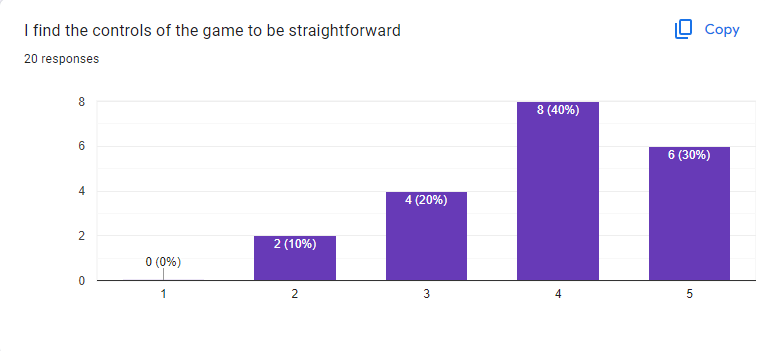
\includegraphics[scale=0.7]{Capstone/docs/VnVReport/StraightForward.png}}
\label{fig:StraightForward}
\end{figure}

\begin{figure}[htbp]
\caption{Navigation Usability Survey Results}
\centerline{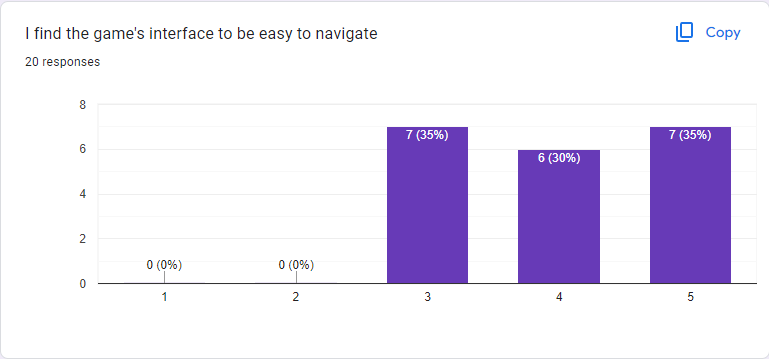
\includegraphics[scale=0.7]{Capstone/docs/VnVReport/Navigation.png}}
\label{fig:Navigation}
\end{figure}

\begin{figure}[htbp]
\caption{Detached Usability Survey Results}
\centerline{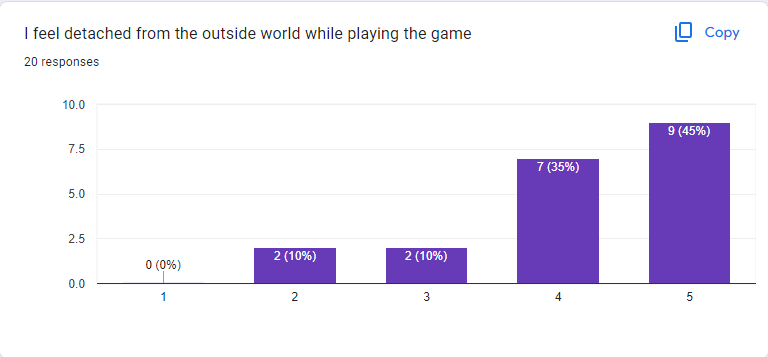
\includegraphics[scale=0.7]{Capstone/docs/VnVReport/Detached.png}}
\label{fig:Detached}
\end{figure}

\begin{figure}[htbp]
\caption{Real World Usability Survey Results}
\centerline{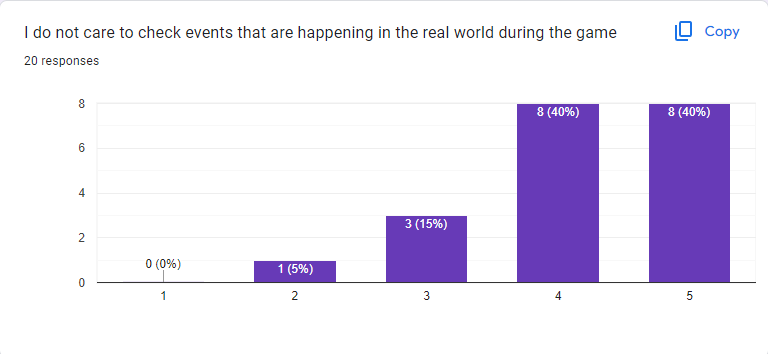
\includegraphics[scale=0.7]{Capstone/docs/VnVReport/RealWordl.png}}
\label{fig:RealWorld}
\end{figure}

\begin{figure}[htbp]
\caption{Fun Usability Survey Results}
\centerline{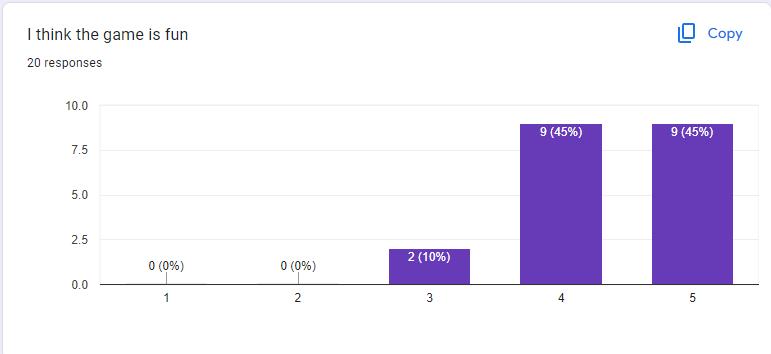
\includegraphics[scale=0.7]{Capstone/docs/VnVReport/Fun.png}}
\label{fig:Fun}
\end{figure}

\begin{figure}[htbp]
\caption{Social Usability Survey Results}
\centerline{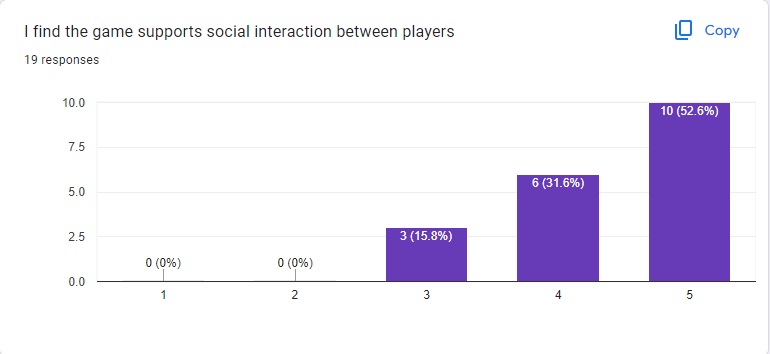
\includegraphics[scale=0.7]{Capstone/docs/VnVReport/Social.png}}
\label{fig:Social}
\end{figure}

\begin{figure}[htbp]
\caption{Enjoyment Usability Survey Results}
\centerline{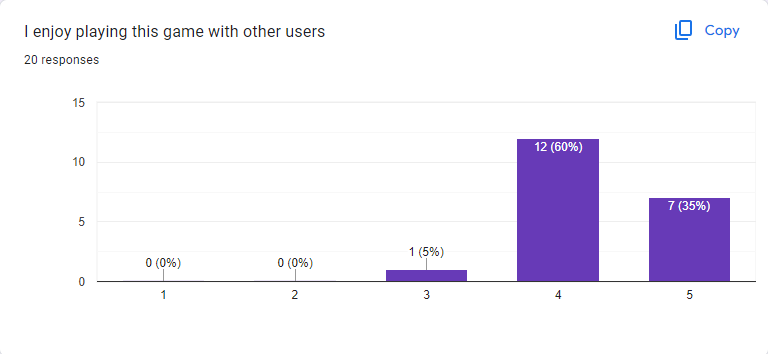
\includegraphics[scale=0.7]{Capstone/docs/VnVReport/Enjoy.png}}
\label{fig:Enjoy}
\end{figure}

\begin{figure}[htbp]
\caption{Imagination Usability Survey Results}
\centerline{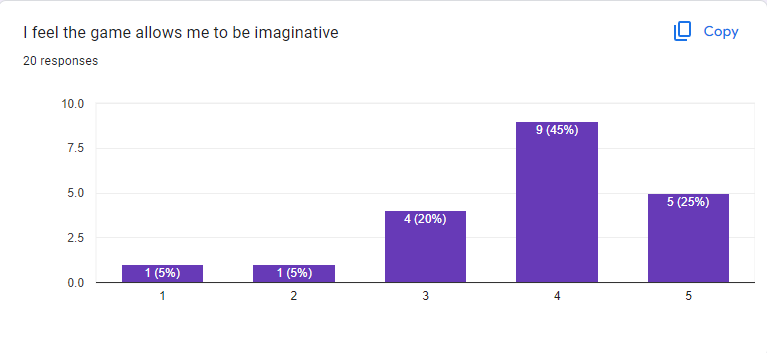
\includegraphics[scale=0.7]{Capstone/docs/VnVReport/Imagination.png}}
\label{fig:Imagination}
\end{figure}

\begin{figure}[htbp]
\caption{Challenging Usability Survey Results}
\centerline{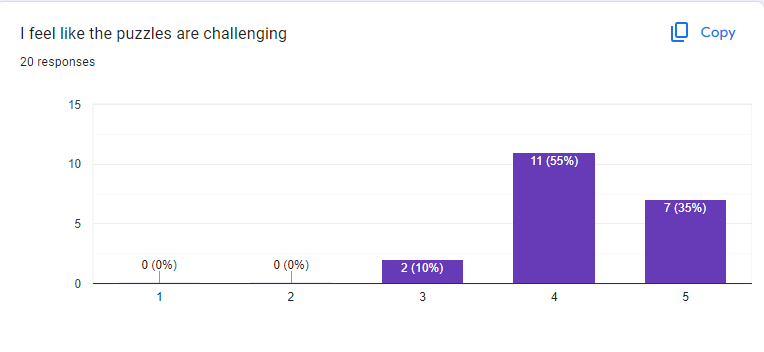
\includegraphics[scale=0.7]{Capstone/docs/VnVReport/Challenging.png}}
\label{fig:Challenging}
\end{figure}

\begin{figure}[htbp]
\caption{Puzzle Interactions Usability Survey Results}
\centerline{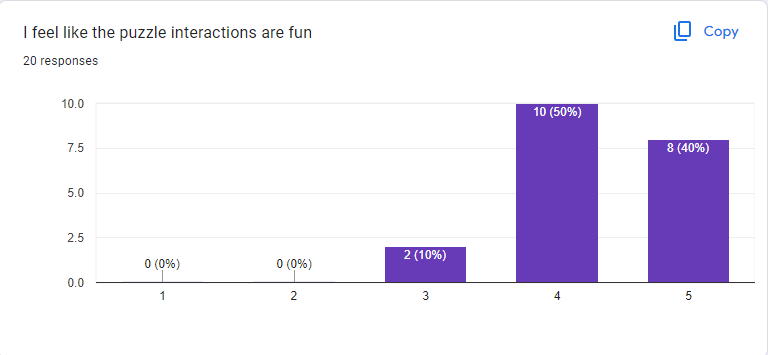
\includegraphics[scale=0.7]{Capstone/docs/VnVReport/PuzzleInteractions.png}}
\label{fig:PuzzleInteractions}
\end{figure}

\begin{figure}[htbp]
\caption{Graphics Interactions Usability Survey Results}
\centerline{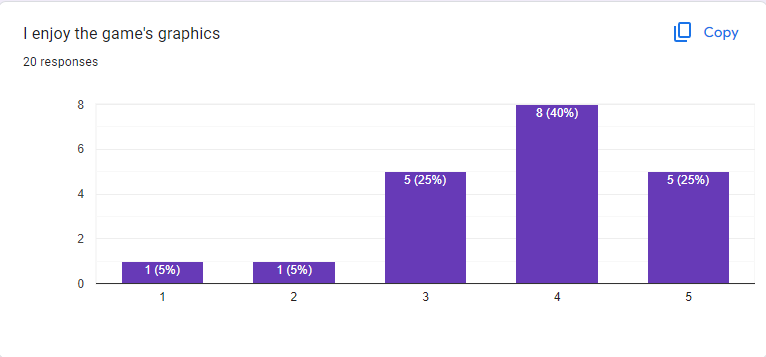
\includegraphics[scale=0.7]{Capstone/docs/VnVReport/Graphics.png}}
\label{fig:Graphics}
\end{figure}

\begin{figure}[htbp]
\caption{VisuallyAppealing Interactions Usability Survey Results}
\centerline{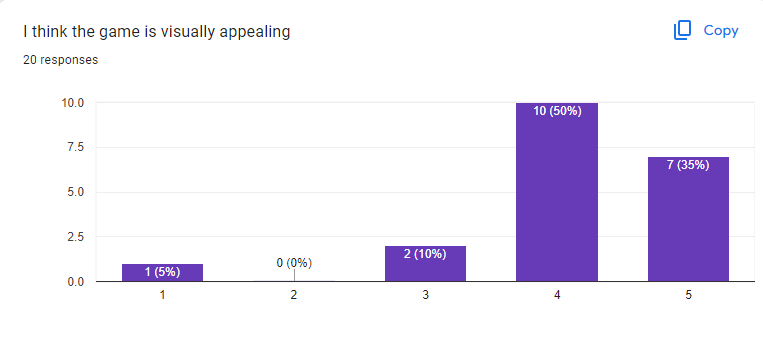
\includegraphics[scale=0.7]{Capstone/docs/VnVReport/VisuallyAppealing.png}}
\label{fig:VisuallyAppealing}
\end{figure}




\end{document}